% This is "Rapport-Paper" 
% Adapted from "sig-alternate.tex" V2.1 April 2013
% This file should be compiled with V2.5 of "sig-alternate.cls" May 2012
%
% This .tex file (and associated .cls V2.5) produces:
%       1) The Permission Statement
%       2) The Conference (location) Info information
%       3) The Copyright Line with ACM data
%       4) NO page numbers
%
% This .tex source is an example which *does* use
% the .bib file (from which the .bbl file % is produced).
% REMEMBER HOWEVER: After having produced the .bbl file,
% and prior to final submission, you *NEED* to 'insert'
% your .bbl file into your source .tex file so as to provide
% ONE 'self-contained' source file.
%
% ================= IF YOU HAVE QUESTIONS =======================
% Questions regarding the SIGS styles, SIGS policies and
% procedures, Conferences etc. should be sent to
% Adrienne Griscti (griscti@acm.org)
%
% Technical questions _only_ to
% Gerald Murray (murray@hq.acm.org)
% ===============================================================
%
% For tracking purposes - this is V2.0 - May 2012
\documentclass{sig-alternate}

% PREAMBLE
% This is "Include.tex"
\usepackage[USenglish, american]{babel}
\usepackage{ucs}
\usepackage[utf8x]{inputenc} 							% Encoding (allows accents)
\usepackage{epstopdf}
\usepackage[printonlyused,nolist]{acronym}	% Acronyms (print only used)

\newlength{\wideitemsep}
\setlength{\wideitemsep}{\itemsep}
\addtolength{\wideitemsep}{+10pt}
\newcommand{\tallitem}{\setlength{\itemsep}{\wideitemsep}\item}
\usepackage{bm}
\usepackage{breqn}

\usepackage{forest} % for diagrams
\usepackage{tikz-qtree} % for digrams
\usepackage{pgf-umlsd} %uml diagrams
\usepackage{cite}
\usepackage{float}
\usepackage{interval}

\newcommand{\specialcell}[2][c]{%
  \begin{tabular}[#1]{@{}l@{}}#2\end{tabular}}
  
  
  
  % XML

\definecolor{dkgreen}{rgb}{0,0.6,0}
\definecolor{gray}{rgb}{0.5,0.5,0.5}
\definecolor{mauve}{rgb}{0.58,0,0.82}
\definecolor{gray}{rgb}{0.4,0.4,0.4}
\definecolor{darkblue}{rgb}{0.0,0.0,0.6}
\definecolor{lightblue}{rgb}{0.0,0.0,0.9}
\definecolor{cyan}{rgb}{0.0,0.6,0.6}
\definecolor{darkred}{rgb}{0.6,0.0,0.0}

% XML

\usepackage{listings}
\usepackage{xcolor}

\lstset{
  basicstyle=\ttfamily\footnotesize,
  columns=fullflexible,
  showstringspaces=false,
  numbers=left,                   % where to put the line-numbers
  numberstyle=\tiny\color{gray},  % the style that is used for the line-numbers
  stepnumber=1,
  numbersep=5pt,                  % how far the line-numbers are from the code
  xleftmargin=20pt,
  framexleftmargin=15pt,
  backgroundcolor=\color{white},      % choose the background color. You must add \usepackage{color}
  showspaces=false,               % show spaces adding particular underscores
  showstringspaces=false,         % underline spaces within strings
  showtabs=false,                 % show tabs within strings adding particular underscores
  frame=shadowbox,                   % adds a frame around the code
  rulecolor=\color{black},        % if not set, the frame-color may be changed on line-breaks within not-black text (e.g. commens (green here))
  tabsize=3,                      % sets default tabsize to 2 spaces
  captionpos=b,                   % sets the caption-position to bottom
  breaklines=true,                % sets automatic line breaking
  breakatwhitespace=false,        % sets if automatic breaks should only happen at whitespace
  title=\lstname,                   % show the filename of files included with \lstinputlisting;
                                  % also try caption instead of title  
  commentstyle=\color{gray}\upshape
}


\lstdefinelanguage{XML}
{
  morestring=[s][\color{mauve}]{"}{"},
  morestring=[s][\color{black}]{>}{<},
  morecomment=[s]{<?}{?>},
  morecomment=[s][\color{dkgreen}]{<!--}{-->},
  stringstyle=\color{black},
  identifierstyle=\color{lightblue},
  keywordstyle=\color{red},
  morekeywords={xmlns,xsi,noNamespaceSchemaLocation,type,id,x,y,source,target,version,tool,transRef,roleRef,objective,eventually}% list your attributes here
}
\graphicspath{{figures/}}

\begin{document}

% Copyright
%\setcopyright{acmcopyright}
%\setcopyright{acmlicensed}

%------------------------------
%HERE
%\setcopyright{rightsretained}
%\insertACM
%------------------------------


%\setcopyright{usgov}
%\setcopyright{usgovmixed}
%\setcopyright{cagov}
%\setcopyright{cagovmixed}

% UID Metadata
% DOI
%\doi{10.475/123_4}

% ISBN
%\isbn{123-4567-24-567/08/06}

% Conference Info

%------------------------------
%HERE
%\conferenceinfo{HRI '17}{June 6--9, 2017, Vienna, Austria}
%------------------------------


%\acmPrice{\$15.00}

% --- Author Metadata here ---
%\conferenceinfo{WOODSTOCK}{'97 El Paso, Texas USA}
%\CopyrightYear{2007} % Allows default copyright year (20XX) to be over-ridden - IF NEED BE.
%\crdata{0-12345-67-8/90/01}  % Allows default copyright data (0-89791-88-6/97/05) to be over-ridden - IF NEED BE.
% --- End of Author Metadata ---

% This is the ACRONYMS Definition
\begin{acronym}[H.264/SVC]
	\acro{API}{Application Program Interface}
	\acro{HD}{High Definition}
	\acro{HDTV}{High Definition Television}
	\acro{IP}{Internet Protocol}
	\acro{IT}{Information Technology}
	\acro{LAN}{Local Area Network}
	\acro{OS}{Operating System}
	\acro{P2P}{Peer-to-Peer}
	\acro{TCP}{Transport Control Protocol}
	\acro{UDP}{User Datagram Protocol}
	\acro{UI}{User Interface}
	\acro{URL}{Uniform Resource Locator}
	\acro{WLAN}{Wireless Local Area Network}
	\acro{XML}{Extensible Markup Language}
	\acro{IST}{Instituto Superior Técnico}
	\acro{NLP}{Natural Language Processing}
	\acro{POS}{Part-of-speech}
	\acro{SVM}{Support Vector Machine}
	\acro{ME}{Maximum Entropy}
	\acro{ML}{Machine Learning}
	\acro{GAIPS}{Intelligent Agents and Synthetic Characters Group}
	\acro{IPL}{Iterative Perceptual Learning}
	\acro{PCS}{Parasocial Consensus Sampling}
	\acro{SVM}{Suport Vector Machine}
	\acro{HRI}{Human-Robot Interaction}	
	\acro{NLP}{Natural Language Processing}	
	\acro{WoZ}{Wizard-of-Oz}
	\acro{IRI}{Interpersonal Reactivity Index}
	\acro{CRF}{Conditional Random Field}
	\acro{SERA}{Socially Expressive Robotics Architecture}
	\acro{AI}{Artificial Intelligent}
	\acro{ROS}{Robot Operating System}
	\acro{RL}{Reinforcement Learning}
	\acro{EMYS}{EMotive headY System}
	\acro{IRI}{Interpersonal Reactivity Index}
	\acro{VHT}{Virtual Human Toolkit}
	\acro{ASAP}{Artificial Social Agent Platform}
	\acro{FAtiMA}{Fearnot AffecTIve Mind Architecture}
	\acro{BML}{Behaviour Markup Language}
	\acro{MDP}{Markov Decision Processes}
	\acro{SAL}{Sensitive Artificial Listeners}
	\acro{FML}{Function Markup Language}
	\acro{GUI}{Graphical User Interface}
	\acro{SSI}{Social Signal Interpretation}
	\acro{AU}{Action Unit}
	\acro{WPF}{Windows Presentation Foundation}
	\acro{TTS}{Text-To-Speech}
\end{acronym}

\title{Rapport}
\subtitle{Establishing Harmonious Relationships Between Robots and Humans}


%\numberofauthors{5}
\numberofauthors{1}
\author{
% 1st. author
\alignauthor Bruno Henriques \\
       \affaddr{Instituto Superior Técnico}\\
       \affaddr{Lisbon, Portugal}\\
       \email{bruno.p.henriques@tecnico.ulisboa.pt}
% 2nd. author
%\alignauthor Nuno Xu\\
%       \affaddr{Instituto Superior Técnico}\\
%       \affaddr{Lisbon, Portugal}\\
%       \email{nuno.xu@tecnico.ulisboa.pt}
%% 3rd. author
%\alignauthor Tiago Ribeiro\\
%       \affaddr{INESC-ID}\\
%       \affaddr{Instituto Superior Técnico}\\
%       \affaddr{Lisbon, Portugal}\\
%       \email{tiago.ribeiro@gaips.inesc-id.pt}
%\and
%% 4th. author
%\alignauthor Rui Prada\\
%       \affaddr{INESC-ID}\\
%       \affaddr{Instituto Superior Técnico}\\
%       \affaddr{Lisbon, Portugal}\\
%       \email{rui.prada@gaips.inesc-id.pt}
%% 5th. author
%\alignauthor Ana Paiva\\
%       \affaddr{INESC-ID}\\
%       \affaddr{Instituto Superior Técnico}\\
%       \affaddr{Lisbon, Portugal}\\
%       \email{Ana.Paiva@inesc-id.pt}
}

% ---------------------------------------------------------------------------------------------------------------
\maketitle
% This is "Abstract.tex"

\begin{abstract}

Autonomous agents are becoming our next companions. They may be able to offer physical therapy assistance, play games and even help us treat weight loss. However, it is not enough to build agents that create strong first impressions. They need to continuously convey such feelings and encourage user interactions, i.e., to build and maintain rapport over long periods of time. In order to manage rapport, agents need to show signs of positivity, mutual attention and coordination during, e.g., motivate, establish eye contact, and postural mimicry, respectively. Nowadays, social agents only tackle one of these components, and the ones that do are not robotic. For this purpose, we designed an extensible rapport model that enables robotic and virtual agents to show natural signs of rapport according to the dyadic state of the interaction. The model was implemented using the \acf{SERA} ecosystem and tested using robot \ac{EMYS} on a novel scenario called Quick Numbers regarding likeability, intelligence, animacy, and proximity. There is no statistical significance on the obtained results, however, from the video footage, we noticed that the participants manifested more positive reactions and emotions in the rapport condition, therefore, a sample higher than 20 might reveal the expected statistical results. Finally, researchers may integrate the rapport model on any \ac{SERA} agent with low effort.

\end{abstract}

%------------------------------
%HERE
%% This is "CSSXML.tex"
%
% The code below should be generated by the tool at
% http://dl.acm.org/ccs.cfm
%

\begin{CCSXML}
<ccs2012>
<concept>
<concept_id>10003120.10003121</concept_id>
<concept_desc>Human-centered computing~Human computer interaction (HCI)</concept_desc>
<concept_significance>500</concept_significance>
</concept>
<concept>
<concept_id>10010147.10010178.10010219.10010221</concept_id>
<concept_desc>Computing methodologies~Intelligent agents</concept_desc>
<concept_significance>500</concept_significance>
</concept>
<concept>
<concept_id>10010147.10010178.10010216.10010217</concept_id>
<concept_desc>Computing methodologies~Cognitive science</concept_desc>
<concept_significance>300</concept_significance>
</concept>
<concept>
<concept_id>10010147.10010341.10010349.10010355</concept_id>
<concept_desc>Computing methodologies~Agent / discrete models</concept_desc>
<concept_significance>300</concept_significance>
</concept>
</ccs2012>
\end{CCSXML}

\ccsdesc[500]{Human-centered computing~Human computer interaction (HCI)}
\ccsdesc[500]{Computing methodologies~Intelligent agents}
\ccsdesc[300]{Computing methodologies~Cognitive science}
\ccsdesc[300]{Computing methodologies~Agent / discrete models}

%
% End generated code
%
%------------------------------

% --------------------------------------------------------
%\printccsdesc
\keywords{\ac{HRI}; Rapport; Rapport; Framework; \acf{SERA}; \acf{EMYS}}
% --------------------------------------------------------
% This is "Introduction.tex"

\begin{figure*}
	\centering
	%\begin{framed}
		\scalebox{0.85}{
            \begin{forest}
                [\textbf{Build Rapport}
                    [Stimulate Positivity 
                        [Self-disclosure][Motivate][Humor]]
                    [Stimulate Mutual Attention
                        [Mutual Gaze][Backchannel]]
                    [Stimulate Coordination
                        [Behavioural Mimicry
                            [Facial Expressions][Head Gestures]]
                        [Adhere To Social Norms]
                        [Backchannel]]
                ]               
            \end{forest}
        }
	%\end{framed}
	\caption{Example of a goal tree to build rapport. The nodes are goals and the leafs are actions.}
	\label{table:BuildingRapportPlan}
\end{figure*}

\section{Introduction}
\label{sec:Introduction}

Robots are increasingly becoming part of our society and their presence has been proven to impact our lives. But do any of us remember a remarkable interaction with a robot to the same degree we are able to recall one with a person? What makes one conversation memorable? 

In order to answer these questions, researchers have been exploring agents capable of building rapport, i.e., designing agents that consider the following aspects during interactions: positivity, mutual attention, and coordination~\cite{Spencer-Oatey2005}. In reality, most of the today's agents do not consider formally this concept, and yet they have been impacting people's lives on several scenarios such as education~\cite{Burroughs2007}, child care~\cite{Burns1984} and medical assistance~\cite{Kang2005, Lisetti2013}. Researchers have been mostly considering single aspects of rapport such as gaze~\cite{Andrist2015, Mutlu2006, Stanton2014, Andrist2014, Baxter2014, Wang2010} and backchannel~\cite{Truong2011, Huang2010, Poppe2011, Poppe2010, Kok2012, Niewiadomski2009} (listener behaviour), which is not enough, as rapport is managed more efficiently when considering its three components. More importantly, we only found virtual agent capable of managing these three components~\cite{Buschmeier2011, Gratch2006}. 

This work tackles the lack of robotic agents capable of building rapport using its three components. For this purpose, we designed and implemented a rapport model (Sections~\ref{sub:rapportModel} and ~\ref{sec:model_implementation}, respectively) on robot \ac{EMYS} using the \ac{SERA} ecosystem~\cite{Tullio2015}. The designed rapport model enables concurrent execution of rapport behaviours using a prioritisation mechanism where idle actions (e.g., postural mimicry) have lower priorities than behaviours triggered momentarily (e.g., surprise animations). These strategies may be either rule-based or \ac{ML}-based but they all cooperate to achieve the interactional goals of the scenario.

To analyse the performance of the developed rapport strategies, we conducted user studies to study its impact on likeability, intelligence and liveness using Godspeed questionnaires~\cite{bartneck2009measurement, lehmann2015good}, and proximity~\cite{aron1992inclusion} using the Quick Numbers scenario detailed in Section~\ref{sec:studies}.
\section{Background}
\label{sec:Background}

For the following sections, the main concepts of the document will be described. Section~\ref{subsec:Rapport} describes the concept of rapport since it is the main phenomenon we want to elicit on people's perception. Currently, researchers have been starting to use \acl{ML} approaches which Section~\ref{subsec:Rapport} describes. Lastly, Section~\ref{subsec:ReinforcementLearning} describes \acl{RL} \ac{ML} techniques, following current suggestions made by several researchers~\cite{Thomaz2006, Kok2012, Sequeira2016, Zhao2014, Papangelis2014}.

\subsection{Rapport}
\label{subsec:Rapport}
The feeling of flow and connection during interactions is formally known as rapport~\cite{Wang2009}. It is a phenomenon that affects people on three levels: emotional, behavioural and cognitive~\cite{Wang2009}.

The emotional level refers to the impact the relationship has on partners, while behavioural refers to, for example, the convergence of movements and facial expressions. Finally, the cognitive level refers to a shared understanding between conversational partners~\cite{Wang2009}.

Spender Oatey~\cite{Spencer-Oatey2005} suggests that rapport management can be divided into three main tasks: enhancement, maintaining and destroy. The first task aims to create strong first impressions, the second encourages the continuation and the third task aims to destroy relationships. Each one of these tasks can be modelled as abstract goals that can be accomplished by achieving sub-goals only satisfied by interacting with the external world~\cite{Papangelis2014, Zhao2014} (see Figure~\ref{table:BuildingRapportPlan}). These sub-goals manipulate the three components of rapport suggested by Tickle-Degnen and Rosenthal~\cite{Tickle-Degnen1990}:

\begin{itemize}
	\item \textbf{Positivity}: feeling of approval and friendliness (e.g. head nod and smile);
	\item \textbf{Mutual attention}: feeling that the other's attention is focused on the individual (e.g. mutual gaze and ``hmm hmm'' vocalisations);
	\item \textbf{Coordination}: feeling of predictability and being in-sync (e.g. postural mimicry and synchronised movements).
\end{itemize}

\vspace{-5mm}
\begin{figure}
	\centering
	%\begin{framed}
		\scalebox{0.65}{
			\begin{forest}
				[\textbf{Build Rapport}
				[Stimulate Positivity 
					[Elicit Positive emotions [Smile] [Embarrassed Laugh][Praise]]]
				[Stimulate Mutual Attention
					[Mutual Gaze] [Voice utterances][Paraphrasing]]
				[Stimulate Coordination
					[Postural Mirror]
					[Be predictable
						[Adhere To Social Norms
							[Greet] [Be Polite]]]]
				]
			\end{forest}
		}
	%\end{framed}
	\caption{Example plan for building rapport. The nodes are goals and the leafs are actions.}
	\label{table:BuildingRapportPlan}
\end{figure}
\vspace{-4mm}

However, in order to build rapport, it is essential that these three components co-exist during an interaction~\cite{Grahe1999, Wang2010, Zhao2014, Cassell2007}. For example, using gaze to establish mutual attention conveys disinterest and can have negative social effect if not accompanied by other behaviours that stimulate positivity and coordination~\cite{Wang2010}. Although, the relative weights of these components may change as the relationship evolves beyond strangers~\cite{Wang2010, Zhao2014, Cassell2007}.

Moreover, two strangers behaviours are initially driven by cultural conventions as they do not know each other and, therefore, they expect what was taught by their cultural environment according to the current context~\cite{Zhao2014} (e.g. greet and be polite). As the relationship evolves and the interlocutors get to know one another, positivity decreases and it is replaced by coordination while mutual attention remains constant~\cite{Zhao2014, Tickle-Degnen1990}. The interlocutors may even violate what is culturally accepted in order to meet interactional goals and behavioural expectations~\cite{Zhao2014}. For example, friends may use sarcasm and insults instead of politeness~\cite{Zhao2014}. Table~\ref{table:rapportStrategies} describes examples of verbal and non-verbal strategies for managing rapport.

\vspace{-3mm}
\begin{table}[]
	\centering
	\begin{tabular}{@{}ll@{}}
		\toprule
		\multirow{2}{*}{\textbf{Verbal}}    & Humour; Paraphrasing; Self disclosure; Praise; Ego Suspension.\\ 
		& Refer to shared experience; Slower rate of speech; Small-talk; \\ \midrule
		\multirow{2}{*}{\textbf{Non-verbal}} & Gaze; Smile; Reciprocate previous action. Silence; Postural mimicry; \\  
		& Gesture mimicry; Mirror Facial Expression; Head gestures. \\ \bottomrule
	\end{tabular}
	\caption{Examples of strategies and actions to manage rapport.}
	\label{table:rapportStrategies}
\end{table}
\vspace{-8mm}

Learning behavioural expectation is also important to assess rapport success. This can be achieved through the use of self-disclosure \cite{Moon2000}, small-talk~\cite{Cassell2003} and humour~\cite{Treger2013}. For instance, when self-disclosure is successful, it is reciprocal, intimacy increases, disclosed topics become more diversified, and deeper~\cite{Zhao2014}. Moreover, assessing when rapport strategies were successful is also important, for example, mutual gaze and smiling become more noticeable and consistent\cite{Grahe1999, Zhao2014}.

To sum up, rapport is a phenomenon that makes interactions more engaging and harmonious. Rapport management can be modelled as a problem of goal satisfaction that is solved through the realisation of actions. However, the strategies for managing rapport must take into account the goals of the interaction and the sociocultural context of the interaction in order to satisfy behavioural expectations. Although, these expectations may not be clear at first and strategies for learning them should be applied.
\subsection{\acl{ML}}
\label{subsec:MachineLearning}

\acf{ML} is a subfield in Computer Science that develops algorithms capable of automatically learn and make predictions based on data~\cite{Bishop2006}. In supervised learning, the data is retrieved from datasets or corpus, and in unsupervised learning, the data is directly sampled from the interaction. Despite not requiring handcrafted rules, these algorithms requires large amounts of quality data and good discriminative features in order to create good predicting models or classifiers. However, acquiring great amount of data may prove difficult in \ac{HRI} since it takes a great toll on the development design as it requires careful preparation, feature selection, data processing techniques, and most of all, test subjects (Figure~\ref{fig:MLDiagram}).

In addition, preliminary studies, in the intended scenario, are crucial to assess the most relevant interactions, and behavioural features we have to look before starting the training stage (see relation between the dataset and training in Figure~\ref{fig:MLDiagram}). One must take into account that excessive features may lead to redundancy (noise) contributing negatively to the quality of the classifier (overfitting). Therefore, it is recommended to use less features in order to have better generic model.

% REMOVED ADDED IF I HAVE SPACE (HALF PAGE)
%Most \ac{ML}-algorithms use eager learning techniques where the models produce global approximations to the given dataset however, there are another algorithms (e.g., $k$-nearest neighbours) that use lazy learning~\cite{Atkeson1997} to produce local approximations. These algorithms store the training dataset locally that is only used when given a test sample. Depending on the intended scenario, the latter approach may return better results. For example, eager learning may model a graph curve using a liner function (global approximation) whether lazy learning may use several liner functions (local approximations).


\begin{figure}[hbt]
  \centering
  %\begin{framed}
	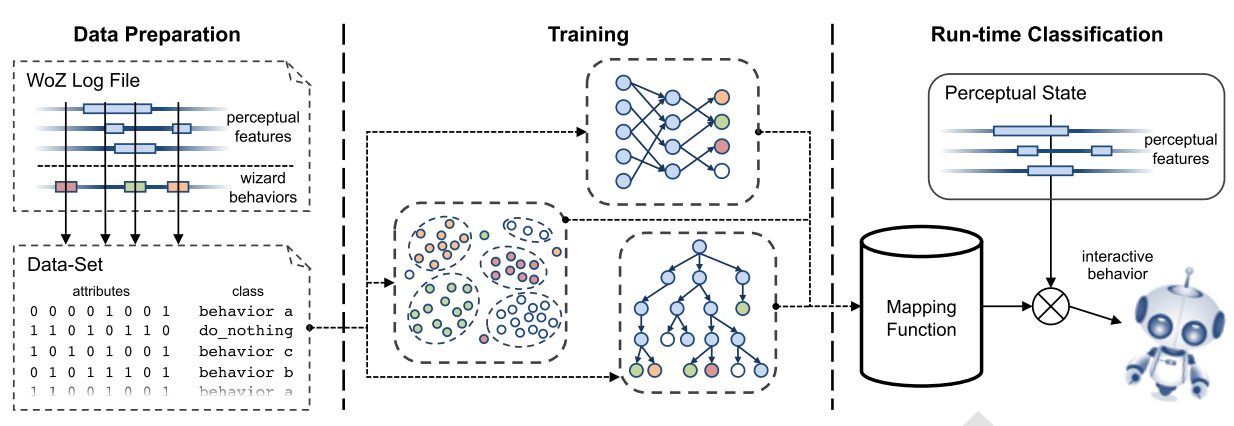
\includegraphics[width=\textwidth]{images/RestrictedPerception_ML_Diagram.png}
  %\end{framed}
  	\caption{Illustration of a \ac{ML} system in a \ac{HRI} application. The dataset is collected and prepared, then it is given to a \ac{ML} algorithm, and lastly, in run-time, the mapping function returns the most appropriate response given an input. From~\cite{Sequeira2016}.}
  	\label{fig:MLDiagram}
\end{figure}
\vspace{-3mm}

Finally, the predictive models' performance are tested using data that were not used during the training stage (test set and training set respectively). In order to limit overfitting issues, model validation techniques such as cross validation are used to test if the classifier is sufficiently generic to any given independent test dataset.

Usually, in supervised learning, the performance is measured regarding the precision (Equation~\ref{eqn:precision}) and recall (Equation~\ref{eqn:Recall}) of the generated output according to the what is expected in the corpus (TP, FP, and FN stands for True Positives, False Positives, and False Negatives, respectively).

\vspace{-9mm}
\begin{multicols}{2}
	\begin{equation}
		Precision = \frac{TP}{TP + FP}
		\label{eqn:precision}
	\end{equation}\break
	\begin{equation}
		Recall = \frac{TP}{TP + FN}
		\label{eqn:Recall}
	\end{equation}
\end{multicols}
\subsection{Reinforcement Learning}
\label{subsec:ReinforcementLearning}

\acf{RL} is sub-field in \ac{ML} that guides agents' actions, in an environment, to maximise a cumulative reward~\cite{Sutton:1998:IRL:551283, Dayan1992}. \ac{RL} systems contain:

\begin{itemize}
	\item A set of possible world states $S$;
	\item A set of possible actions $A$;
	\item Transitioning rules between states;
	\item A immediate reward function $R(s,s',a)$ with $a \in A$, and $s,s' \in S$;
	\item Rules to describe the environment.
\end{itemize}

Typically, these systems deal with environments where the optimal reward function might not be clear~\cite{Sutton:1998:IRL:551283}. To tackle this issue, \ac{RL} agents uses exploration strategies to find the best policy function $\pi(s)$ that returns the most probable action $a \in A$, given a state $s \in S$, that maximises the cumulative reward (Equation~\ref{eq:policy}). In social behaviours, agents that are eager to interact with its partner (instead of being silent) will acquire more information regarding it's performance during interactions and will be able to learn more quickly as they test new different interactional strategies.

\vspace{-3mm}
\begin{equation}
	\pi(s) = a,\,a \in A\, and\,s \in S
	\label{eq:policy}
\end{equation}

One well researched \ac{RL} algorithm is Q-Learning~\cite{Dayan1992}. In Q-Learning, the virtual agents learns and stores Q-Values that depends on the reward value for a given action $R(s_t,a_t,s_{t+1})$, on an estimation of future reward $\max_{a}Q(s_{t+1},a)$, on the learning rate $\alpha_t \in {[0,1]}$, and on the discount value $\gamma \in {[0,1]}$ (Equation~\ref{eq:QLearning}). The learning rate $\alpha_t$ defines the weight of old information during learning, and the discount value $\gamma$ defines the weight of future rewards.

\vspace{-4mm}
\begin{equation}
	Q(s_t,a_t) = (1-\alpha_t)Q(s_t,a_t) + \alpha_t\left[R(s_t,a_t,s_{t+1}) + \gamma\max_{a}Q(s_{t+1},a)\right]
	\label{eq:QLearning}
\end{equation}

The Q-Values can be zero at the beginning of the learning process, meaning that the agent's does not have previous, or, value different than zero, meaning the the agent has previous knowledge~\cite{Malfaz2011}. The values for $\alpha$ and $\gamma$ are defined according to the developed scenario, the purposes of the agents and overall quality of the final \ac{RL} model.

Lastly, there are two main issues when using \ac{RL}: identifying the reward function and gathering data to satisfy the combinatorial explosion of environment features and possible actions. To solve the first issue, authors suggest extracting the reward function from human experts during demonstrations using inverse \ac{RL}~\cite{Ng2000, Thomaz2006}. That is, collect feedback from human experts regarding the virtual agent's performance and use the information collected to define a reward function. To solve the second issue, the model should take into account fewer environment features and actions.
\fancychapter{Related Work}
\label{chap:relatedwork}

This chapter presents the state of the art related to this work. Since there is a lack of rapport agent studies, the following chapter will focus on agents that are capable, to some extent, of managing rapport.

\subsection{Theoretical Models of Rapport for Agents}
\label{sub:sec:ComputationalModelsOfRapport}

Rapport is a mostly unconscious phenomenon~\cite{Zwiers2011} that occurs during interactions marked by strong perceptions of coordination, positivity and mutual attention.

The most important concepts for managing rapport are: planning social behaviours (Figure~\ref{table:BuildingRapportPlan}), learning social behaviours and flexible mechanisms to regulate current actions. Rapport models involve several complex cognitive mechanisms. Therefore it is beneficial to discretise it into smaller sets capable of, for example, enhancing positivity (friendliness) using self-disclosure or enhancing coordination and attentiveness through backchannel and turn-taking strategies~\cite{Sacks1974, Kahn2008, Welbergen2012}. The latter strategies are allied with good listeners as they must able to understand how to provide well-timed adequate feedback (backchannel) and identify appropriate moments to become the speaker (turn taking) and incite further dialogue~\cite{Sacks1974, Poppe2010}.

Zhao, Papangelis, and Cassell, propose a theoretical model to manage long-term rapport~\cite{Zhao2014, Papangelis2014} that is very relevant for current implementations of long-term social companionship agents~\cite{Lisetti2013, Bickmore2005, Kang2005}. Similarly to what was described previously in Section~\ref{subsec:Rapport}, the proposed model treats rapport as an interactional goal that is satisfied through strategies and actions according to the current state of the interaction and the user model (See Table~\ref{table:TCArchitectureDyadicRapportManagement:State}).

The strategies and the selected actions, despite initially representing the general sociocultural norms, must adapt to the interpersonal norms of the relationship and the context~\cite{Zhao2014}. As the relationship evolves, the dyadic state and the internal models should be updated in order to store the most accurate description of the interaction and return better behavioural responses that satisfy the dyad behavioural expectations~\cite{Papangelis2014}.

\vspace{-3mm}
\begin{table}[]
    \centering
    \begin{tabular}{@{}ll@{}}
        \toprule
        
        \multirow{1}{*}{\textbf{Dyadic State}} & Rapport State; Behavioural model; Friendship Status; History \\ \midrule
        \multirow{2}{*}{\textbf{User Model}} & User goals; Shared knowledge; Task model; \\  
        & Conversational Agent putative dyadic state \\ \bottomrule        

    \end{tabular}
    \caption{Relevant data structures for rapport models. Adapted from~\cite{Zhao2014}.}
    \label{table:TCArchitectureDyadicRapportManagement:State}
\end{table}
\vspace{-7mm}

Another important aspect for managing rapport is the ability to continuously adapt to the current interaction and context, give incremental feedback~\cite{Kopp2007, Zwiers2011, Reidsma2011, Visser2014}, and even recover from mistakes~\cite{Kahn2008}. Its usefulness is remarked on complex synchronised behaviours such as speech and handshakes~\cite{Zwiers2011}. This requires bidirectional connections between the behaviour realisers and the behaviour planners to enable quicker corrections~\cite{Reidsma2011}. This also requires incremental planning and execution of behavioural chunks that can be potentially interrupted, modified or even replaced~\cite{Reidsma2011, Visser2014, Kopp2007, Zwiers2011}. This approach moves away from the typical SAIBA model~\cite{Kopp2006} and requires extending the current \ac{BML}~\cite{Kopp2007, Zwiers2011, Reidsma2011} specifications.
\subsection{Creating Rapport Agents using Rule-Based Approaches}
\label{sub:sec:rulebasedAgents}

In the context of the document, we consider rule-based systems as systems that use rules implicitly or explicitly. For example, the former mimics head gestures using motion sensors and the latter generates backchannel behaviours if the conversational partner pauses his speech for more than one second. Rule-based systems are great for deterministic scenarios where the agent does not need to be as robust as other systems used in non-deterministic scenarios~\cite{Mutlu2006} where rules might not be easy to define. However, these systems are not easily ported to other scenarios, nor are they easily scalable because they are often based on non-trivial conditions~\cite{Kok2012}, and are often specifically tailored to discrete scenarios.

Mutlu et al., implemented a scripted mutual gaze agent that synchronises gaze behaviour with pre-recorded voice and gestures~\cite{Mutlu2006}. In their experience, they concluded that participants would recall the story better when the robot looked at them more. Additionally, using the same gaze frequency, women felt better when the storytelling agent gazed less at them. This is important if we want to develop agents for education scenarios where transmitting information is crucial.

Stanton et al., developed a robot assistant for a cooperative visual tracking game (the ``shell game'')~\cite{Stanton2014}. Volunteers would ask the robot for help. However, occasionally, the robot would volunteer to give an answer. In their experiment, they concluded that eye gaze can have powerful effects upon participant decision-making and behaviour, and influence their task performance. For example, humans tend to comply to the robot's suggestion when it gazed at them on harder tasks but, on easier tasks, gaze reduced trust. The authors postulates that ``robot gaze can have either a positive or negative impact upon trust and compliance, depending upon the nature of the robot’s request or suggestion''.

Andrist et al., developed a virtual agent focused on mutual-gaze behaviour in a therapy scenario~\cite{Andrist2015} that would systematically swap its gazing target between the task area and the conversational partner's using tracking sensors. According to their study, matching gaze behaviour models to the user's personality increases motivation and engagement in repetitive tasks. In other words, different personalities require different rules. For example, between tasks, when therapists would provide encouragement, introverts shift more often their gaze to the therapist than extroverts.

%Chidambaram \textit{et al.}, developed a robotic agent to study the impact of vocal and bodily cues in persuasion~\cite{Chidambaram2012} on Desert Survival Tasks~\cite{30} using gaze, gestures, vocal cues and even proximity to the user. In their findings, they concluded that the presence of non-verbal behaviours impacts people's compliance while and that vocal cues do not. However, the study was made on a hypothetical scenario and it was
\section{Creating Rapport Agent using Data-Driven Based Approaches}
\label{sec:datadrivenbasedAgents}

Rule-based systems are not easily scalable knowing that it is impossible to program an agent to handle every possible situation and outcome, especially when interacting with the unpredictability of human behaviour. Therefore, some scenarios may benefit from having agents capable of adapting to changes in the external world and generate more appropriate social behaviour using data-driven models through several \ac{ML} approaches. Despite not being used actively by this thesis systems, it is fundamental to mention current research work on this area as it is proving invaluable to create agents capable of producing more natural behavioural in comparison with simpler rule-based systems.

\subsection{Supervised Learning}
In supervised learning, the algorithms infer a function from a labelled training set that contains both the input set and the corresponding target value. 

Kok et al., developed an iterative data-driven rapport model focused on generating timings for backchannel behaviours in a dyadic conversational setting~\cite{Kok2012}, \ac{IPL}. The distinctive aspect is the usage of perceptual (subjective) evaluation to identify the moments of the interaction that are perceived as socially inappropriate. In the perceptual evaluation, multiple subjects evaluate the agent's behaviours by pressing a \textit{Yuck} button whenever they would rate each one as socially inappropriate (\ac{PCS})~\cite{Huang2010, Poppe2011}. The resulting model takes into consideration that different listeners have different personalities and that some social behaviours are not mandatory and, therefore not socially inappropriate if they do not occur. This sample retrieval contrasts with the typical corpus-based backchannel models, as in the latter the negative samples are retrieved randomly as long as they do not overlap with the positive samples marked in the corpus~\cite{Kok2012}. Following Figure~\ref{fig:ipl_system}, the typical corpus-based approach is used as the baseline~\cite{DeKok2011} (yellow area) that will be refined with every sequence of generation of behaviour (pink area), subjective evaluation (blue area) and finally training (green area). The resulting model was perceived more natural when compared with the tradition corpus-based approach, however, the authors suggest extending their work with more relevant features from rapport (e.g., mutual gaze, head angles and smiles).

\begin{figure}
	\centering
	\includegraphics[width=0.3\textwidth]{images/IPL_system.png}
	\caption{Schematic representation of the \ac{IPL} framework. From~\cite{Kok2012}.}
	\label{fig:ipl_system}
\end{figure}

\subsection{Unsupervised Learning}

In unsupervised learning, as opposed to supervised, the data does not contain the target value, therefore, the algorithms will try to cluster the data into groups regardless of their meaning.

Mohammad et al., propose a model for interactive robots that can learn how to interact naturally with human conversational partners in different environments and contexts~\cite{Mohammad2010} using unsupervised learning. One of the tested successful scenarios was learning how to apply backchannels in a dyadic setting with a human instructor. According to their results, the backchannel behaviour generation was more natural, performing better than the traditional rule-based, however, there is no comparison regarding the traditional supervised learning approaches.

\subsection{Active Learning}
In active learning, the algorithms interact to seek knowledge regarding how to classify an instance with a label~\cite{Bishop2006}.

Cakmak, Thomaz and colleagues have been researching the potential of active learning on agents that actively seek information and fill gaps in their knowledge, potentially improving their performance~\cite{Chao2010, Cakmak2010, Cakmak2012, Thomaz2006}. In their studies, they noticed that people who better understand the agent's queries are able to train the model with ``perfect accuracy relatively quickly'' and had more confidence on the trained model performance~\cite{Chao2010}. However, previous work has been more focused on learning task-related information and not, learning better interactional models to build and maintain rapport.

Moreover, it is important to properly design the experiments to correctly collect data. For example, Thomaz et al., developed an agent using reinforcement learning \cite{Thomaz2006}. During the experiment, despite asking the humans not to provide feedback (only guidance), they influenced the results. As the author describes ``people use the reward signal to give anticipatory rewards or future directed guidance for the agent''.

\subsection{\acf{WoZ}}
\label{subsec:woz}
In \acf{WoZ} studies~\cite{Steinfeld2009}, subjects are led to believe that they are interacting with an autonomous robot when, in fact, they are interacting with a human (the wizard). Following the current trend of using \ac{WoZ} studies~\cite{Steinfeld2009} to train virtual agents~\cite{Knox2014, Mutlu2006} to be more socially competent, Pedro Sequeira et. al. propose a methodology for discovering interaction strategies from restricted-perception \ac{WoZ} studies~\cite{Sequeira2016}. In restricted-perception \ac{WoZ}, the wizard's perceptions and actions are limited to the same extent as the agent enabling a better learning environment and better resemblance to the studies environment~\cite{Sequeira2016}. The set of perceptions and actions are collected using mock-up studies. The disadvantage of this approach is that it requires more preparation than the unrestricted \ac{WoZ} and, even then, it might be impossible to completely isolate the wizard's perceptions.
\section{Creating Rapport Agents using Hybrid Approaches}

Recently, researchers are exploring hybrid agents that combine the advantage of rule-based systems to define high-level interaction rules that are triggered by simpler perceptual states and data-driven models to generate behaviour according to more complex situations that may emerge during interactions.

Pedro Sequeira et. al. proposes the usage of mock-up studies and the previously mentioned restricted-perception \ac{WoZ} (Section~\ref{subsec:woz}) to develop a Hybrid Controller that takes advantage of rule-based systems and \ac{ML}-based systems in a tutoring scenario~\cite{Sequeira2016}. Following Figure~\ref{fig:RestrictedPerception_DesignProcess}, the inherent agent's limitations are defined in the \textit{Task AI} to be used on the restricted-perception \ac{WoZ} Studies. The hybrid controller is based on the expert knowledge and the \ac{WoZ} data collected during the previous stage, and is responsible for deciding when and which behaviour to trigger. For example, a rule-based component would trigger a summarisation of the main achievements during the game and another \ac{ML}-based component would trigger actions that were learnt during the restricted-perception \ac{WoZ} studies (recall that the wizards controls ``which interaction behaviour should be triggered and when to trigger it''~\cite{Sequeira2016}). In the last stage, \textit{Strategy Refinement}, \ac{HRI} researchers assess the agent's performance and refines the controller if necessary for situations that may not have been properly learned or, for situations that require more relevant information.

\begin{figure}[H]
	\centering
	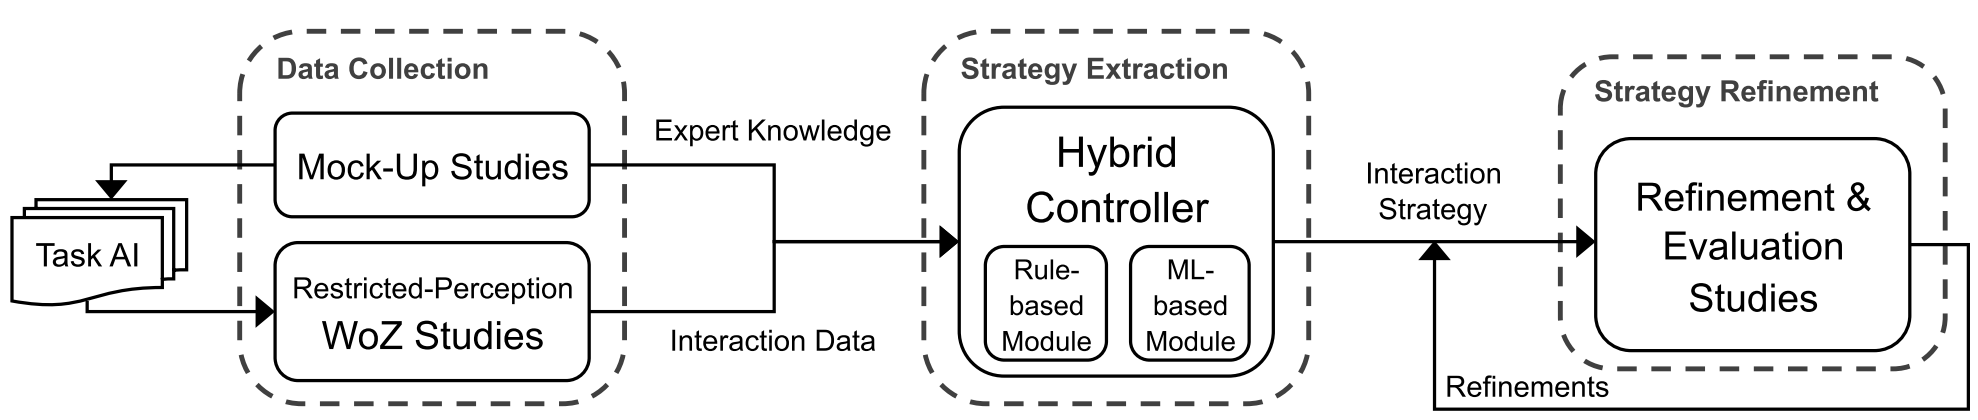
\includegraphics[width=0.85\textwidth]{images/RestrictedPerception_DesignProcess.png}
	\caption{Restricted-perception \ac{WoZ} study methodology. From~\cite{Sequeira2016}.}
	\label{fig:RestrictedPerception_DesignProcess}
\end{figure}




\subsubsection{Virtual Rapport 2.0} \hspace*{\fill} \\
\label{sub:sec:virtualrapport2}

Huang et al., developed a short-term rapport agent to enhance mutual attention and coordination using backchannels through a data-driven approach that takes into account context-specific response models in a dyadic conversational setting~\cite{Buschmeier2011}. The model determines the best suitable timings to generate specific backchannel behaviours and turn-taking opportunities according to the perceptual state observed.

%%%%%%%%%%%%%%%%%%%%%%%%%%%%%%%%%%%%%%%%%%%%%%%%%%%%%%%%%%%%%%%%%%%%%%%%%%%%%%%%%%%%%

\paragraph{\textbf{System description}}

Following Figure~\ref{fig:virtualrapport2System}, the system contains the following modules:
\begin{itemize}
	\item \textbf{\textit{Perception}}: analyses human speaker's behaviour in real time;
	\item \textbf{\textit{Response Models}}: predicts timing of backchannel feedback and end-of-turn opportunities in real time using information from the environment and from the agent itself. It also decides which behaviour to generate;
	\item \textbf{\textit{Generation}}: generates the output from the response models;	
	\item \textbf{\textit{Consensus Data}}: contains data collected from Rapport 06-07 dataset and Self-disclosure data-set (\url{http://rapport.ict.usc.edu}) using \ac{PCS}. The data contains dyadic interactions between a human speaker telling a story and human silent listener.
\end{itemize}

\begin{figure}[hbt]
  \centering
  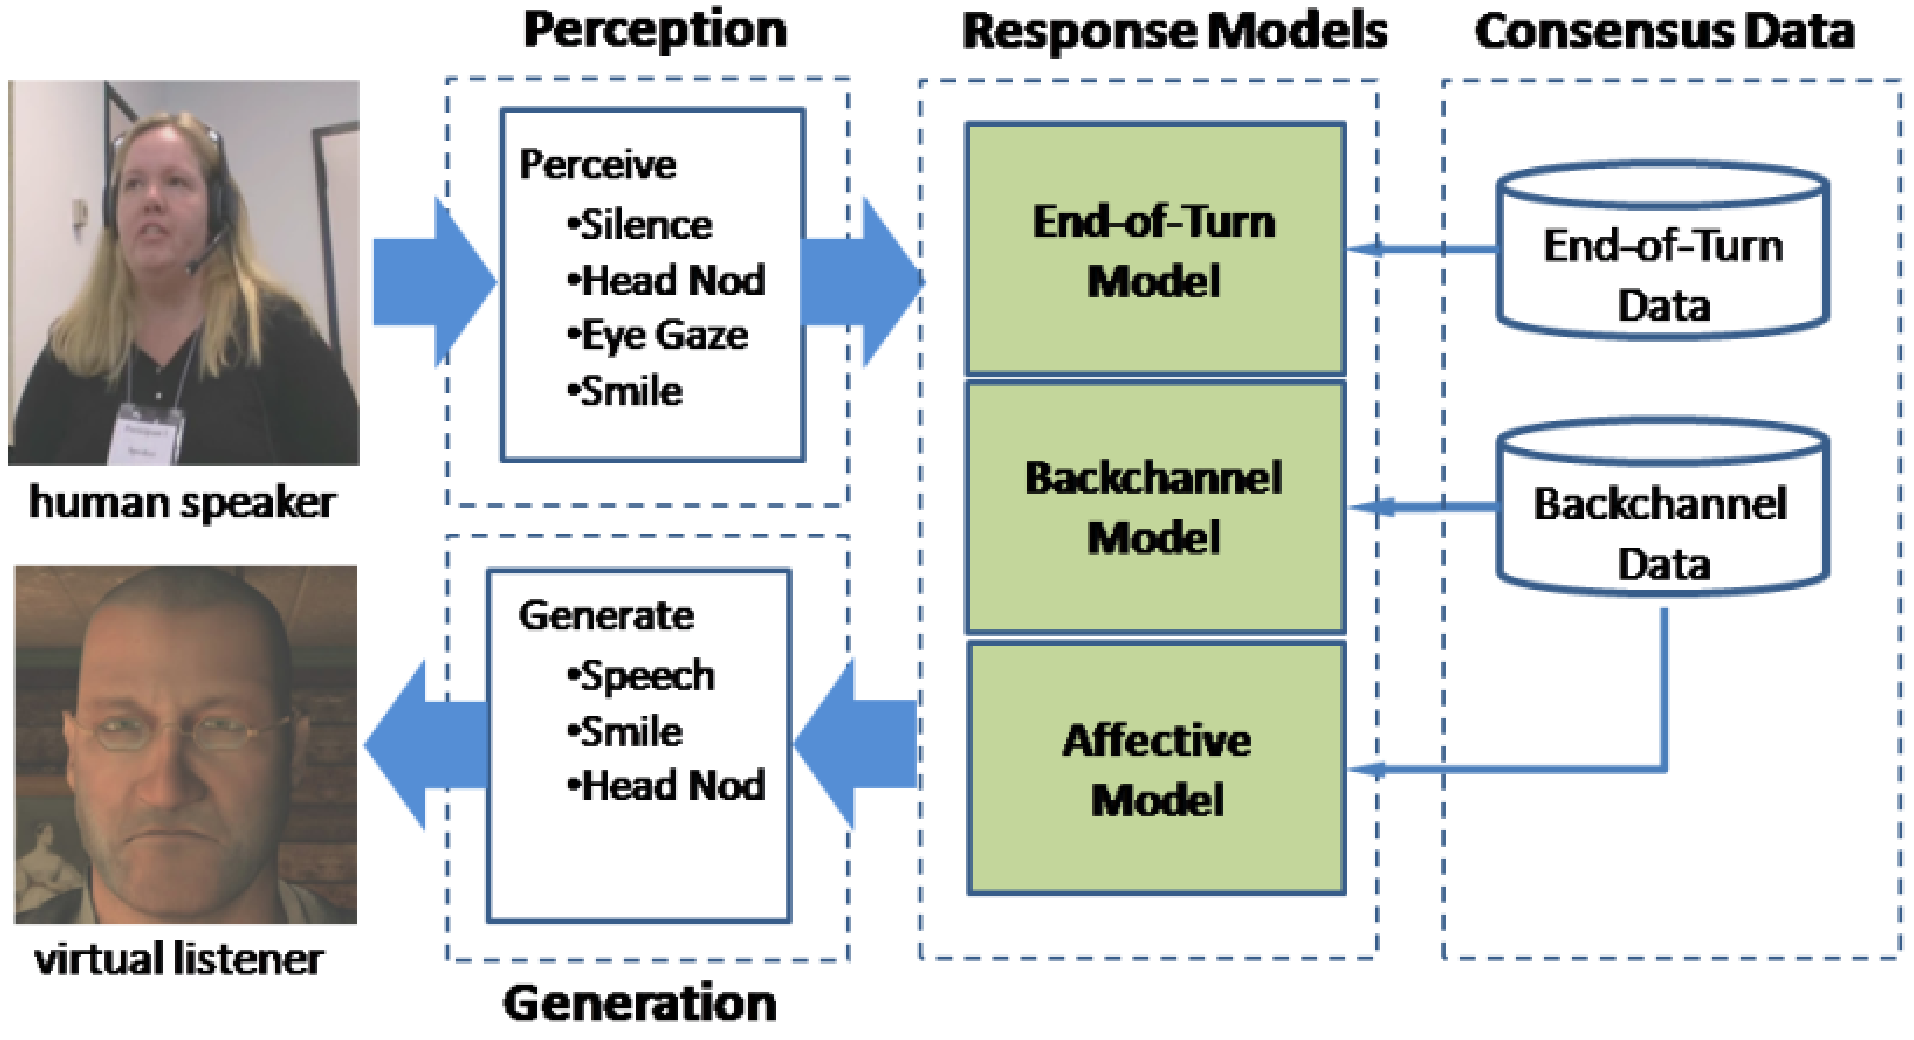
\includegraphics[width=0.8\textwidth]{images/VirtualRapport2_System.png}
  \caption{Architecture of Virtual Rapport 2.0: The \textit{Perception} module analyses human behaviour in real time. \ac{PCS} data is used to create the \textit{Response Models} module. Lastly, the output of the models is generated by the \textit{Generation} module. From~\cite{Buschmeier2011}.}
  \label{fig:virtualrapport2System}
\end{figure} 

As depicted in Figure \ref{fig:virtualrapport2System} there are three models in the \textit{Response Models} module: \textit{End-of-turn}, \textit{Backchannel}, and \textit{Affective}.

The first model, \textit{end-of-turn}, using a rule-based approach, identifies turn-taking opportunities by analysing the current speaker's non-verbal behaviours. For example, if the human interrupts the virtual agent, the agent stops, yields his turn and, says ``I am sorry, keep going'' while showing a facial expression~\cite{Buschmeier2011}.

The second model, \textit{Backchannel}, is \ac{ML}-based (using forward-only inference \ac{CRF} for real-time predictions) and trained using the Rapport 06-07 dataset. It is capable of predicting when and how to give non-verbal feedback.

The last model, \textit{Affective}, analyses facial feature points in real time and detects whenever the speaker is smiling.
 
During the interaction, the three response models are used in conjunction to decide whenever it is appropriate to generate a backchannel. If the speaker is smiling (according to the \textit{Affective} model) and if it is a good opportunity to generate a backchannel (according to the \textit{Backchannel} model) then a head nod (one of the three identified in their studies) is generated accompanied by a smile.

%%%%%%%%%%%%%%%%%%%%%%%%%%%%%%%%%%%%%%%%%%%%%%%%%%%%%%%%%%%%%%%%%%%%%%%%%%%%%%%%%%%%%%%%

\paragraph{\textbf{Evaluation}}
The developed virtual agent interacted with the human subjects in a interview environments in which the former was the interviewer and the later the interviewed. With the goal of comparing the developed system with the previous version~\cite{Gratch2006}, the evaluation measured the following dimensions: rapport (five-item social presence scale~\cite{Bailenson2001}), overall naturalness, backchannel feedback and end-of-turn prediction.


%%%%%%%%%%%%%%%%%%%%%%%%%%%%%%%%%%%%%%%%%%%%%%%%%%%%%%%%%%%%%%%%%%%%%%%%%%%%%%%%%%%%%%%%

\paragraph{\textbf{Discussion}}
The results demonstrates a significant improvement over the previous version. Over 90\% of the users preferred the Virtual Rapport 2.0 rapport agent over the previous rule-based system~\cite{Gratch2006, Morency2008}. The timing's precision and recall are much better, leading to a better synchronism and perceived naturalness from the user during the interaction. According to the authors, the data-driven design, the much richer set of emotions capable of mimicking smiles, and the generation of more natural head gestures might explain the overall better results on the stronger feelings of rapport.

To conclude the most relevant aspects of the system are:
\begin{itemize}
	\item Corpus based approach;
	\item Identification of different head nods patterns;
	\item Duality of \ac{ML}-bases decision and smile to generate backchannel behaviour;
	\item Creative strategy for handling interruptions.
\end{itemize}
\subsubsection{\acl{SAL}} \hspace*{\fill} \\
\label{subsec:AutonomousSensitiveArtificialListeners}

Schröder et al. developed a virtual agent integrated in SEMAINE~\cite{Schroder2010} called \ac{SAL} that has the required capabilities to sustain conversational dialogues and be a good listener~\cite{Schroder2012}.

\paragraph{\textbf{System Description}}

Following the representation of the \ac{SAL} system in Figure~\ref{fig:sensitiveAgent}, the most relevant components are: \textit{Feature extractors}, \textit{Analysers}, \textit{Interpreters}, \textit{Action proposers}, and \textit{Action selection}. The \textit{Feature extractors} component extracts several features such as head gestures, facial features, emotions and, most of all, acoustic features. These features are later analysed by the \textit{Analysers} and \textit{Interpreters} components. The former component analyses non-verbal behaviours and speaker's emotions to produce an estimate of the information's reliability. The later component, given the information available, returns the best state representation for the user, dialogue and agent. Following this, several \textit{Action proposers} will propose an action, in parallel, given previous information. Following, the \textit{Action selection} component selects the action with the highest estimated quality, and lastly, the \textit{Behaviour generator} generates the desired action (utterances and facial animations).

\vspace{-3mm}
\begin{figure}
	\centering
	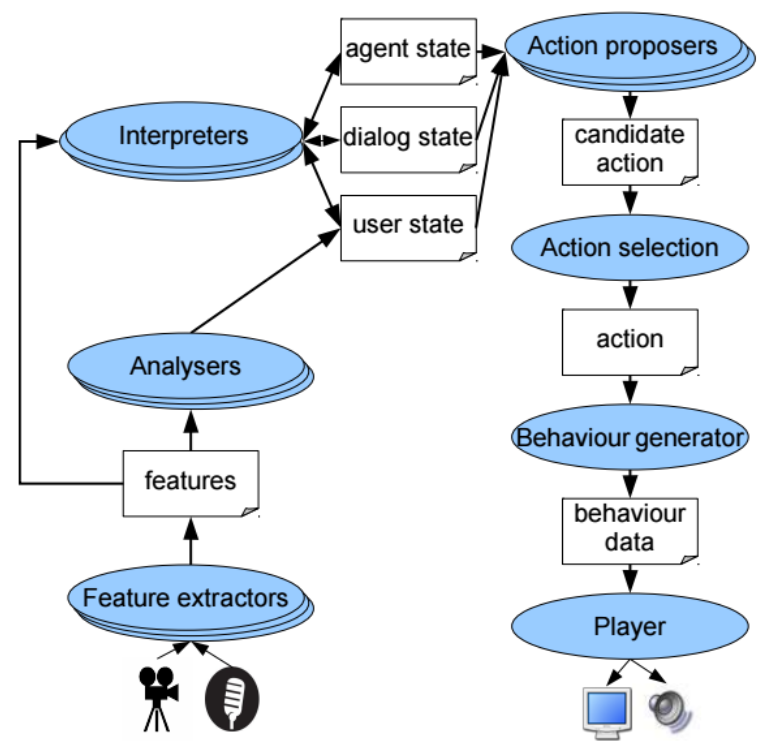
\includegraphics[width=0.5\textwidth]{images/SensitiveAgent.png}
	\caption{\acl{SAL} conceptual architecture. From~\cite{Schroder2012}.}
	\label{fig:sensitiveAgent}
\end{figure}
\vspace{-7mm}

The agent is capable of identifying whether it should be in listener or in speaker mode. This is relevant as the \textit{Action selection} component gives more priority over speaker's actions. An example speaker action would be  saying ``Well?'' or ``Go on, tell me your news!'' after a long pause. In addition, in listener mode, the \textit{Action selection} component chooses the most appropriate backchannel to be produced according to the emotions and interest level estimated from the user.

\paragraph{\textbf{Evaluation}}

The objective was to evaluate if emotion-related abilities influence the quality of human interactions. Firstly the users, with minimal \ac{HRI} experience, receive a introductory briefing on the available personalities they can interact with (4 in total). Then, they can interact twice with each available personality one with the expressive agent, the other with the affective features of the output disabled (randomly). The user interacts with the \ac{SAL} agent's presented in a computer screen (only the face is rendered), using the available cameras and microphones.

\paragraph{\textbf{Discussion}}
There is evidence that expressive abilities may substantially impact the interactions between humans and agents by denoting that flow and perceived engagement was much higher in the emotional \ac{SAL} than in the control environment. Compared with previous described systems, it is one of the most complete models for managing backchannels and turn taking strategies, however, as stated previously in Section~\ref{subsec:Rapport}, attentiveness and coordination are not enough to build rapport, it is also necessary to stimulate positivity which this system does not cover. To conclude, the most relevant aspects of the systems are:

\begin{itemize}
	\item Generate good listeners without understanding semantically what it is being said;
	\item Parallel independent action proposers that uses both rule and \ac{ML} approaches;
	\item Dedicated dialogue management models;
	\item Covers several users affective states by modelling distinct characters.
\end{itemize}
% https://www.lightbluetouchpaper.org/2007/03/14/how-not-to-write-an-abstract/
% http://web.ece.ucdavis.edu/~jowens/biberrors.html

\subsection{Overall Discussion}
\label{subsec:RelWorkDiscussion}

Developing a computational models capable of managing rapport similarly to humans is not an easy feat. Researchers had to focus their research on different aspects of rapport and assess their overall contribution. Table~\ref{fig:comparison:rapportSystems} and Table~\ref{fig:comparison:vh:systems}, respectively, compares the systems regarding how they learn social behaviours, and the used rapport management strategies.

\addtolength{\tabcolsep}{1pt}
\begin{table}
	\centering
	\begin{tabular}{lccccccccccc}
		& \textbf{Type}
		& \textbf{Agent} 
	  	& \rot[70]{\textbf{Gaze}}
	  	& \rot[70]{\textbf{Backchannel}} 
	  	& \rot[70]{\textbf{Small-Talk}} 
	  	& \rot[70]{\textbf{Facial Expressions}}
	  	& \rot[70]{\textbf{Gestures}} 
	  	& \rot[70]{\textbf{Mirroring}} 
	  	& \rot[70]{\textbf{Smile}}
	  	& \rot[70]{\textbf{Turn Taking}}
	  	& \rot[70]{\textbf{Praise}}
	  	\\
	  	\midrule
	  	%%%%%%%%%%%%%%%%%%%%%%%%%%%%%%%%%%%%%%%%%%%%%%%%%%%%%%%%%%%%%%
	  	Mutlu et al.~\cite{Mutlu2006} & Rule-based & Robotic & \cmark & \xmark & \xmark & \xmark & \xmark & \xmark & \xmark & \xmark & \xmark\\
	  	%%%%%%%%%%%%%%%%%%%%%%%%%%%%%%%%%%%%%%%%%%%%%%%%%%%%%%%%%%%%%%
	  	Stanton et al.~\cite{Stanton2014} & Rule-based & Robotic & \cmark & \xmark & \xmark & \xmark & \xmark & \xmark & \xmark & \xmark & \xmark\\
	  	%%%%%%%%%%%%%%%%%%%%%%%%%%%%%%%%%%%%%%%%%%%%%%%%%%%%%%%%%%%%%%
	  	Andrist et al.~\cite{Andrist2015} & Rule-based  & Robotic & \cmark & \xmark & \xmark & \xmark & \cmark & \xmark & \xmark & \xmark & \cmark\\
	  	%%%%%%%%%%%%%%%%%%%%%%%%%%%%%%%%%%%%%%%%%%%%%%%%%%%%%%%%%%%%%%
	  	Mohammad et al.~\cite{Mohammad2010} & \ac{ML}-based  & Robotic & \textbf{?} & \cmark & \xmark & \xmark & \xmark & \xmark & \xmark & \xmark & \xmark \\ 
	  	%%%%%%%%%%%%%%%%%%%%%%%%%%%%%%%%%%%%%%%%%%%%%%%%%%%%%%%%%%%%%%
	  	Huang et al.~\cite{Buschmeier2011} & \ac{ML}-based & Virtual & \xmark & \cmark & \cmark & \cmark & \cmark & \cmark & \cmark & \xmark & \xmark\\
	  	%%%%%%%%%%%%%%%%%%%%%%%%%%%%%%%%%%%%%%%%%%%%%%%%%%%%%%%%%%%%%%
	  	Kok et al.~\cite{Kok2012} & \ac{ML}-based & Virtual &  \xmark & \cmark & \xmark & \xmark & \cmark & \xmark & \xmark & \xmark & \xmark\\
	  	%%%%%%%%%%%%%%%%%%%%%%%%%%%%%%%%%%%%%%%%%%%%%%%%%%%%%%%%%%%%%%
	  	Schröder et al.~\cite{Schroder2012} & \ac{ML}-based & Virtual & \xmark & \cmark & \xmark & \cmark & \cmark & \xmark & \xmark & \cmark & \xmark\\
  		\bottomrule
	\end{tabular}
	\caption{Brief comparison regarding how different virtual agents manage strategies. The systems presented here appear in the same order as in the main body of the text.  \protect\cmark, \protect\xmark \, and \textbf{?}, represents whether the specified strategy is applied, not applied or unclear, respectively.}
	\label{fig:comparison:rapportSystems}
	
\end{table}
\addtolength{\tabcolsep}{-1pt}

Current literature suggests continuing the research on learning social behaviours from \ac{WoZ}~\cite{Sequeira2016, Knox2014, Papangelis2014} studies and use primarily \ac{RL}~\cite{Thomaz2006, Kok2012, Zhao2014, Papangelis2014} classifiers (Section~\ref{subsec:ReinforcementLearning}). This class of algorithms are applicable in rapport as there are sequences of states that will help the agent to know when and how backchannels should be produced in order to build rapport (the reward function). In addition, authors suggest developing solutions capable of adapting current course of actions to the current context of the interaction to improve the quality of virtual agents during interactions~\cite{Kopp2007, Zwiers2011, Reidsma2011, Visser2014}.

\begin{table}[]
	\centering
	\begin{tabular}{|l|c|c|}
		\hline
		\textbf{System}              	& \textbf{Training Source} 	& \textbf{Iterative} \\ \hline
		%%%%%%%%%%%%%%%%%%%%%%%%%%%%%%%%%%%%%%%%%%%%%%%%%%%%%%%%%%%%%%%%%%%%%%%%%%%%%%%%%%%%%%%%%%%%%%%%%
		Mohammad et al.~\cite{Mohammad2010} & Direct Samples (Unsupervised) & Yes \\ \hline
		%%%%%%%%%%%%%%%%%%%%%%%%%%%%%%%%%%%%%%%%%%%%%%%%%%%%%%%%%%%%%%%%%%%%%%%%%%%%%%%%%%%%%%%%%%%%%%%%%
		Virtual Rapport 2.0~\cite{Buschmeier2011} 			& Corpus			& No \\ \hline
		%%%%%%%%%%%%%%%%%%%%%%%%%%%%%%%%%%%%%%%%%%%%%%%%%%%%%%%%%%%%%%%%%%%%%%%%%%%%%%%%%%%%%%%%%%%%%%%%%
		\acf{IPL}~\cite{Kok2012}          				& Corpus \& Subjective evaluation			& Yes \\ \hline
		%%%%%%%%%%%%%%%%%%%%%%%%%%%%%%%%%%%%%%%%%%%%%%%%%%%%%%%%%%%%%%%%%%%%%%%%%%%%%%%%%%%%%%%%%%%%%%%%%
		\acf{SAL}~\cite{Schroder2012} & Corpus \& \ac{WoZ}		& Yes \\ \hline
		%%%%%%%%%%%%%%%%%%%%%%%%%%%%%%%%%%%%%%%%%%%%%%%%%%%%%%%%%%%%%%%%%%%%%%%%%%%%%%%%%%%%%%%%%%%%%%%%%
		Restricted Perception~\ac{WoZ}~\cite{Sequeira2016}  & \ac{WoZ}		& Yes \\ \hline
		
	\end{tabular}
	\caption{Brief comparison of methodologies to learn human social behaviours.}
	\label{fig:comparison:vh:systems}
\end{table}

Most of all, the communication goals of interactions must be considered when developing rapport agents. The context in which the communication partners will interact, the inherent limitations of the virtual agents' perceptions and actions and, most importantly, what kind of emotions and actions we want to elicit from the conversational partner are crucial for the development of such agents. For example, in tutoring applications, mutual gaze plays an important role for increased learning performance \cite{OTTESON1980, SHERWOOD1987, Fry1975}, and in negotiation scenarios not reciprocating negative self-disclosure has ben shown to destroy rapport\cite{Bronstein2012}.




\subsection{\acl{SERA}}
\label{sub:sec:sera}

\acf{SERA} follows asynchronous messaging architecture similar to \ac{ROS}~\cite{Quigley2009} where clients communicate with one another through \textit{Thalamus} network messages. Beside supporting robotic agents, \ac{SERA} provides non-technical researchers the ability to customise the agent's behaviour using mark-up text (Table~\ref{table:exampleutterances}). 

The most important elements of \ac{SERA} are:
\begin{itemize}
	\item \textbf{\textit{Thalamus}}: receives and delivers the published messages to the right subscribers;
	\item \textbf{\textit{Skene}}: translates high-level intentions into actions;
	\item \textbf{\textit{Nutty Tracks}}: animation engine;
	\item \textbf{\textit{Speech Server}}: \ac{TTS} engine. 
\end{itemize}

Effector clients, in order to change agent's behaviour, have to contact \textit{Skene} that processes and redirects the request to the most suitable clients: \textit{Nutty Tracks} for animations and \textit{Speech Server} for utterances. However, despite supporting interruption of actions, \ac{SERA} is not without issues as:
\begin{itemize}
	\item If a speech request arrives while there is one in execution, the \textit{Speech Server} executes them sequentially which can cause unintended repetition of utterances;
	\item There is a noticeable (less than a second) delay between the requests and the effects, as requests pass firstly through \textit{Skene}, \textit{Thalamus} and finally, either \textit{Nutty Tracks} or \textit{Speech Server}.
\end{itemize}

%To sum up, in order to accomplish our goals, the solution needs to reduce the number of network messages, and distribute the \textit{Skene} responsibilities into different independents modules to promote reusability and customisation of behaviours.

\section{Rapport Computational Model}
\label{sub:rapportModel}

%TODO rever esta intro
The model attempts to build rapport following the goal tree illustrated in Figure~\ref{table:BuildingRapportPlan}. It is sufficiently generic and customisable to tailor the agents to different embodiments and/or \ac{HRI} scenarios. Furthermore, the model supports interruption and replacement of actions according to the dyadic state of the interaction, as it is vital to adaptive agents~\cite{Reidsma2011, Visser2014, Kopp2007, Zwiers2011}. For example, stop speaking at any time to give the turn to others to speak, possibly apologising for taking the time for doing it~\cite{Buschmeier2011}. %For this purpose, the rapport strategies should that into account the dyadic state of the interaction.

Following Figure~\ref{fig:rapportModel}, the rapport model has the following components:
\begin{itemize}
    \item \textbf{Dyadic State}: contains information regarding the interactional partner and the environment;
    \item \textbf{Perceptions}: perceptual information;
    \item \textbf{Rapport Effectors}: components that generate signs of rapport by proposing actions to the \textit{Rapport Controller} given the dyadic state of the interaction;
    \item \textbf{Rapport Controller}: manages the received actions proposals.
\end{itemize}

\begin{figure}[H]
	\centering
    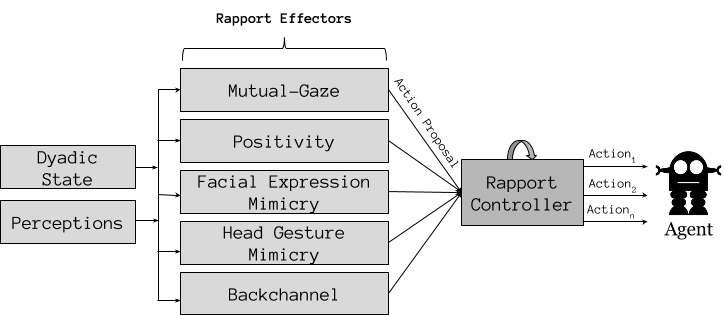
\includegraphics[width=0.48\textwidth]{RapportModel.png}
    \caption{Schematic representation of the rapport model.}
    \label{fig:rapportModel}
\end{figure}

\subsection{Rapport Controller}
\label{sub:sec:modelRapportController}

The \textit{Rapport Controller} manages the proposed actions sent by the different rapport strategies. Each action proposal is a quintuple $A= <G,P,E,I,T>$ containing:

\begin{itemize}
    \item \textbf{Group ($G$)}: part of agent's body that the action is attempting to manipulate;
    \item \textbf{Priority ($P$ where $P \in \mathbb{N}_0$)}: relative importance of the action proposal in relation to others; 
    \item \textbf{Execution description ($E$)}: how the agent will execute the action;
    \item \textbf{Interruption description ($I$)}: how the action should be interrupted by the agent;
    \item \textbf{Timeout ($T$ where $T \in \mathbb{N}$)}: maximum duration.% of the action.
\end{itemize}

Concerning the management of action proposals, the controller periodically captures a snapshot of the agent's ongoing actions and pending action proposals received by the different \textit{Effectors}. Whenever a snapshot is captured or, when receiving a new action proposal, the controller analyses which actions should be interrupted (and replaced). 

\begin{figure}[H]
	\centering
	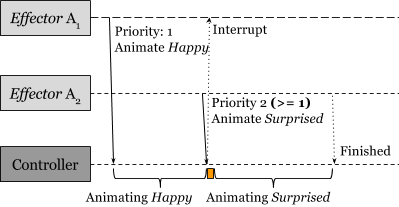
\includegraphics[width=0.38\textwidth]{ConflictingAndInterrupt.png}
	\caption{The action with higher priority interrupts and replaces the action in execution.}	
	%Depiction of an incoming action proposal with different \textit{Group}.
	\label{fig:conflict_interrupt}
\end{figure}

As long as two action proposals, $A$ and $S$, have different groups ($A_G \neq S_G$), both will execute using $A_E$ and $S_E$. However, as illustrated in Figure~\ref{fig:conflict_interrupt}, in the case of a conflict ($A_{1_G}=A_{2_G}$), the action with the highest priority ($A_1$) will interrupt and replace the current one ($A_2$). Moreover, the action can be time limited, therefore, if the action takes longer than expected ($T$) it is interrupted, despite having higher priority. As rule of thumb, idle actions should have a lower priority than actions triggered by discreet states.

\subsection{Stimulate Positivity}

In pursuance of enhancing the first component of rapport, the Positivity rapport\textit{Effector} takes into account the dyadic state of the interaction to trigger vocalisations to motivate, praise, and even humour the interactional partner (Table~\ref{table:positivity_rule_examples}). In addition, the agent should share a personal information to the person (self-disclosure) that plays an important role in closing relationships between two strangers\cite{Kang2011}. 

%The interactional states and the corresponding sentences are specified by the researcher and should tailor to the dyadic state of the interaction as much as possible. For instance, in case of the Portuguese language, which highly inflected on the gender, there have to be distinct sentences for each gender. To conclude, Table~\ref{table:positivity_rule_examples} depicts examples of interactional utterances that the researcher may specify for an agent during a game of Chess.

\begin{table}[H]
	\centering
	\begin{tabular}{|l|l|}
	\hline
	\textbf{Interactional State} & \textbf{Utterance} \\ \hline
	After Introduction & \specialcell{I learnt the castling move today!} \\ \hline
	Player loses the queen & Your king is still well guarded! \\ \hline
	Agent loses a bishop & There goes a bishop! \\ \hline
	\end{tabular}
	\caption{Example utterances depending on the current state of the interaction.}
	\label{table:positivity_rule_examples}
\end{table}

\subsection{Stimulate Mutual Attention}
\label{sub:sec:model_mutual_attention}

Following Figure~\ref{table:BuildingRapportPlan} and~\ref{fig:rapportModel}, the model enhances mutual attention using mutual gaze and backchannel strategies.

The Mutual-Gaze rapport \textit{Effector} bases on the work developed by Andrist et. al.~\cite{Andrist2015}. In short, it swaps between establishing eye contact and looking the game during pre-determined periods of time according to the following conditions: current phase of the scenario (in-task or between-tasks) and the user's personality (introverted or extroverted). The researcher may set the priority of the action proposals, as well as the gaze lengths, which default to the values specified on the work this \textit{Effector} is based on~\cite{Andrist2015}.

The Backchannel \textit{Effector} bases on the work developed by Niewiadomski et. al., on the GRETA system~\cite{Niewiadomski2009} that analyses variations of the pitch to produce listener behaviour. For simplicity, this \textit{Effector} only considers up-down head nods as listener signals. The researcher may set the priority of the generated action proposals, in addition to the trigger probability, the amplitude of the gesture, the gesture velocity, and the number of head nods.

\subsection{Stimulate Coordination}

To enhance coordination, the model uses behavioural mimicry and backchannel strategies.

The Facial Expression Mimicry \textit{Effector} mimics facial expressions (e.g., happiness, surprise, and sadness), triggering animations according to the perceived emotion intensity $I \in \interval{0}{100}$. In addition to the priority of the generated action proposals, the model allows changing the following parameters for each type of emotion: trigger probability, minimum intensity, and priority.

Head Gesture Mimicry \textit{Effector} mirrors head gestures such as up-down nods and left-right shakes ~\cite{Riek2009, Andrist2014, Cassell2007, Wang2009}. In addition to the priority of the generated action proposals, for each gesture, researchers may specify the amplitude, the velocity, and the number of repetitions.

Lastly, the agent should adhere to social norms by, for example, introducing itself when meeting people and saying ``thank you'' when a person does a task for the agent.

%%%%%%%%%%%%%%%%%%%%%%%%%%%%%%%%%%%%%%%%%%%%%%%%%%%%%%%%%%%%%%%%%%%%%%%%%%%%%%%%%%%%%%%%%%

\section{\ac{EMYS}: The Rapport Agent}
\label{sec:model_implementation}

%TODO isto tem potencial para ser cortado
The following section describe the framework that implements the rapport model detailed using \acf{EMYS} robot (Figure~\ref{fig:robots:EMYS2}) as the chosen embodiment to test the rapport agent.

\begin{figure}[H]
	\centering
	\frame{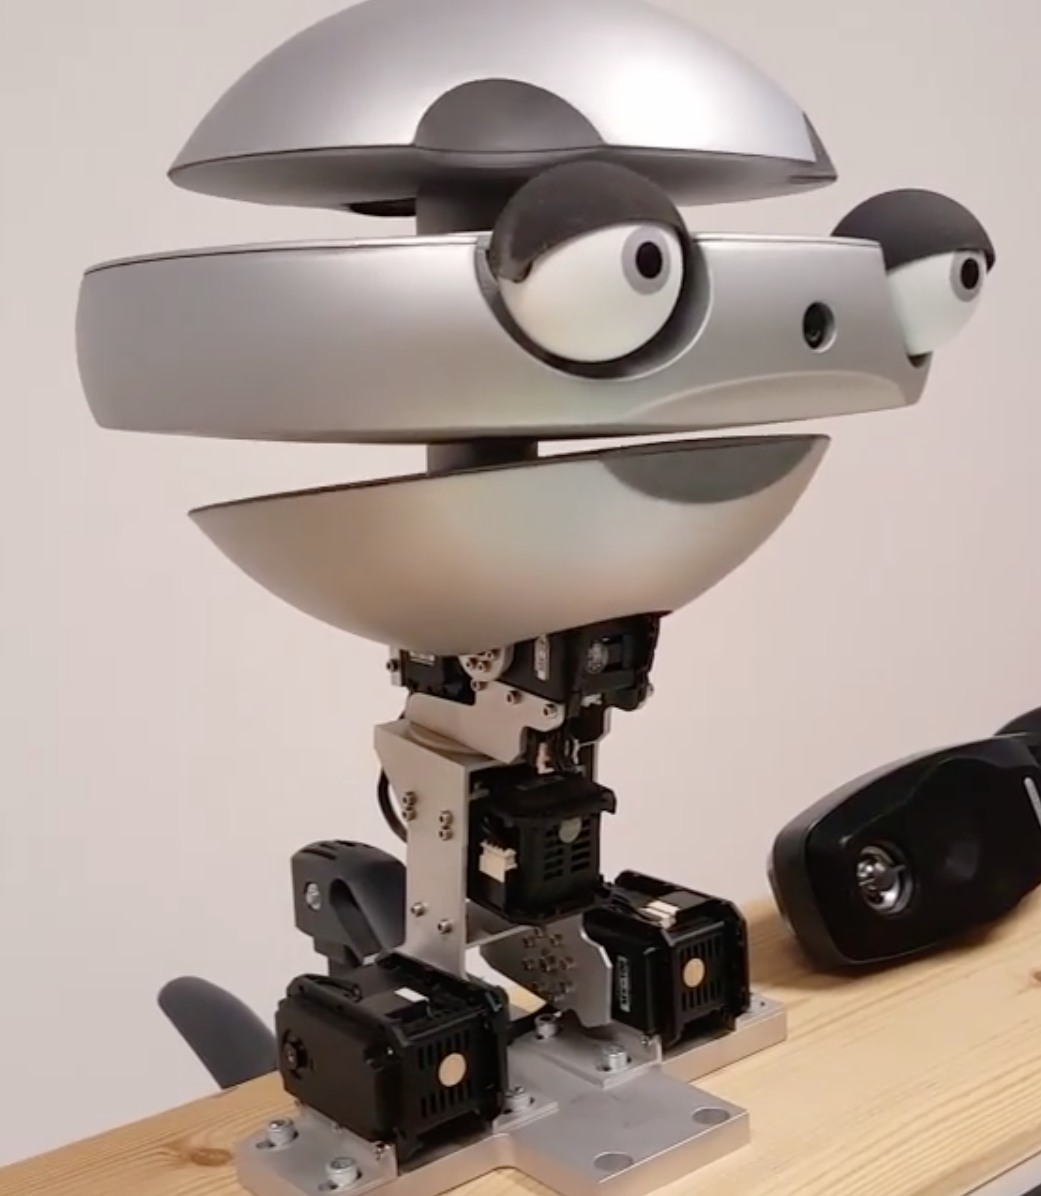
\includegraphics[width=0.1\textwidth]{emys.png}}
	\caption{\ac{EMYS} robot.}
	\label{fig:robots:EMYS2}
\end{figure}

\begin{figure}[H]
	\centering
	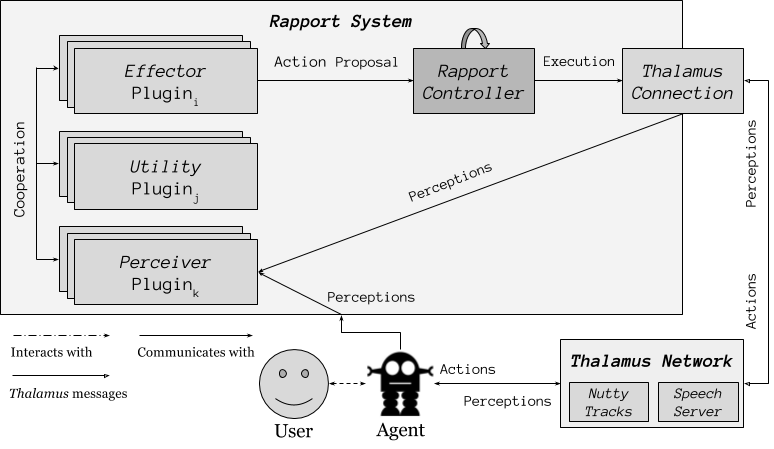
\includegraphics[width=0.47\textwidth]{RapportControllerArchitectureOverview.png}
	\caption{Schematic representation of the framework that implements the rapport model.}
	\label{fig:rapport:archicture}
\end{figure}

The framework follows a plugin-based architecture that, in order to reduce the impact of network delays (Section~\ref{sub:sec:sera}), the internal communication is done using method calls, limiting the number of network messages. Following Figure~\ref{fig:rapport:archicture}, the framework contains the following elements:
\begin{itemize}
	\item \textbf{\textit{Effector Plugins}}: proposes actions and enables/disables plugins;
	\item \textbf{\textit{Perceiver Plugins}}: perceives the external world and informs the interested plugins;
	\item \textbf{\textit{Utility Plugins}}: general purpose plugins that can be used to, for example, store interactional data;
	\item \textbf{\textit{Rapport Controller}}: manages plugins' lifecycle, link plugins, and has the same responsibilities as the rapport model's \textit{Rapport Controller} (Section~\ref{sub:sec:modelRapportController});
	\item \textbf{\textit{Thalamus Connection}}: bridges the system with \ac{SERA}, sending and receiving \textit{Thalamus} messages.
\end{itemize}

The \textit{Cooperation} connection depicted in Figure~\ref{fig:rapport:archicture} establishes the connection between plugins, for example, \textit{Effectors} use \textit{Perceivers} to read perceptual information and may use \textit{Utility} plugins to consult the interaction history. In addition, the \textit{Action} connection is the decisive message that will execute the action proposals defined by the \textit{Effectors} and executed by the \textit{Rapport Controller}.

%The most important connections illustrated in Figure~\ref{fig:rapport:archicture} is 
%Following Figure~\ref{fig:rapport:archicture}, there are five types of connections:
%\begin{itemize}
%	\item \textbf{Perceptions}: perceptual information;
%	\item \textbf{Actions}: the decisive messages that trigger animations or utterances;
%	\item \textbf{Action Proposal}: requests sent by \textit{Effector Plugins};
%	\item \textbf{Execution}: set of actions triggered periodically by the \textit{Rapport Controller} - execution, interruptions or replacement according to the action proposals' stage;
%	\item \textbf{Cooperation}: communication between plugins. For example, for backchannel behaviour, two \textit{Effectors}, one rule-based and one \ac{ML}-based, can cooperate together to trigger the most appropriate social behaviour.
%\end{itemize}


%%%%%%%%%%%%%%%%%%%%%%%%%%%%%%%%%%%%%%%%%%%%%%%%%%%%%%%%%%%%%%%%%%%%%%%%%%%%%%%%%%%%%%%%%%%%%%%%%%

\subsection{Plugins' Lifecycle Management}
\label{sub:sec:pluginLifecycle}

At the startup, the \textit{Rapport Controller} loads the available plugins from a user-selected folder. They are all enabled by default unless specified otherwise through the configuration file that can be accessed using the controller's \ac{GUI} (Figure~\ref{fig:pluginList} in Appendix A). During this process, following Figure~\ref{fig:pluginLifecycle}, each plugin follows a two-step initialisation:

\begin{enumerate}
	\item \textbf{Initialisation}: initialise internal variables;
	\item \textbf{Retrieve Dependencies}: retrieve plugins that it depends on (e.g., \textit{Effectors} typically requires \textit{Perceivers}).
\end{enumerate}

After initialisation, if the \textit{Rapport Controller} is running, \textit{Effectors} can attempt to modify the agent's behaviour concurrently according to the dyadic state of the interaction, until they are disposed of either manually (Figure~\ref{fig:pluginList} in Appendix A), either automatically by another \textit{Effector}. In any case, the plugins are automatically disabled in case of an error without escalating to an application crash.

\begin{figure}[H]
	\centering
	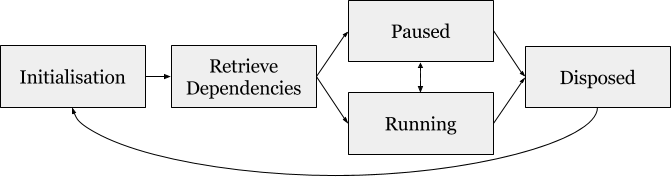
\includegraphics[width=0.47\textwidth]{PluginsLifecycle.png}
	\caption{Plugin's lifecycle.}
	\label{fig:pluginLifecycle}
\end{figure}

\begin{table*}[t]
	\centering
	\begin{tabular}{|l|l|l|l|l|l|}
	\hline
	\multicolumn{1}{|c|}{\textbf{Category}} & \multicolumn{1}{c|}{\textbf{Subcategory}} & \textbf{Utterance}                                                                                      & \textbf{Priority} & \textbf{Delay (ms)} & \textbf{Timeout (ms)} \\ \hline	
	intro & greet & \specialcell{Hi! $<$gaze(person)$>$} I'm EMYS! & 2 & 0 & 30000 \\ \hline
	game & score & \specialcell{Yey! $<$Animate(surprise2, 3)$>$} & 2 & 0 & 30000 \\ \hline
	game & results & \specialcell{Managed $|$\texttt{Points}$|$!\\$<$gaze(person, 3, 500, 5000)$>$} & 2 & 0 & 30000 \\ \hline
	end & ending & \specialcell{Thank you for your participation!\\$<$animate(happy4, 4, 1000)$>$} & 3 & 0 & 30000 \\ \hline		
	\end{tabular}
	\caption{Example compilation of utterances compatible with the developed system. Actions are delimited by $<$ and $>$, and substitution variables by $|$.}
	\label{fig:extended:utterances}
\end{table*}


\subsection{Managing Actions}
\label{sub:sec:managingActions}

The \textit{Rapport Controller} manages action proposals as described in Section~\ref{sub:rapportModel}. However, in addition to the elements of action proposal quintuple $A=<G,P,E,I,T>$, the controller stores the following information:
\begin{itemize}
	\item \textbf{Status}: \textit{pending}, \textit{executing}, \textit{executed} or \textit{interrupted};
	\item \textbf{Starting time}: when the action has started executing; %TODO potential candidate to compact
	\item \textbf{\textit{Thalamus} identifier}: to monitor when actions have finished by monitoring the \textit{Thalamus} messages sent by \textit{Nutty Tracks} and \textit{Speech Server}.
\end{itemize}

The status field is required to manage the state of each action proposal. For example, following Figure~\ref{fig:actionProposalStatus}, an action proposal is only interrupted (using $I$) if its previous state was \textit{executing}. In the absence of the \textit{Thalamus} identifier, we could not flag the actions as executed, making them transition automatically to the \textit{interrupted} state.

\begin{figure}[H]
	\centering
	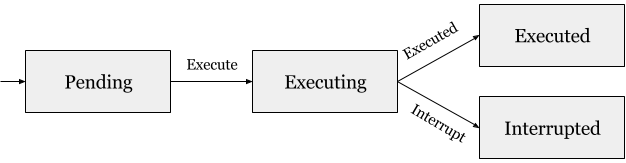
\includegraphics[width=0.47\textwidth]{ActionProposalCycle.png}
	\caption{Action Proposal available states and the corresponding transition graph.}
	\label{fig:actionProposalStatus}
\end{figure}

To conclude, the execution and the interruption descriptions of the action proposal ($E$ and $I$, respectively) are self-contained functions specified by the researcher, therefore they can contain additional logic. However, they must at least send the required \textit{Thalamus} messages to either \textit{Nutty Tracks} or \textit{Speech Server} to produce animations or utterances, respectively.

%%%%%%%%%%%%%%%%%%%%%%%%%%%%%%%%%%%%%%%%%%%%%%%%%%%%%%%%%%%%%%%%%%%%%%%%%%%%%%%%%%%%%%%%%%%%%%%%%%%%%%%%%%%%%%%%%%%%%%%%%%%%%%%%%%%%%%%%%%%%%%%%%%%%%%%%%%%%%%%%%%%%%%%%%%%%%%%%%%%%%%%%%%%%%%%%%%%%%%%%%%

\section{Plugins}
\label{sec:plugins}

There are three types of plugins: \textit{Effectors}, \textit{Perceivers}, and \textit{Utility}. Transparently to the developer, each plugin may specify its \ac{GUI}, and more, importantly, its configuration file (e.g., Listing~\ref{lst:MimicFacialExpressionsSettings}) that allows researchers to tailor the agent's behaviour to the interactional goals of the scenario without having to recompile the code.

%TODO se precisar de espaço, posso tentar compactar isto

\begin{lstlisting}[caption={Excerpt of the \ac{XML} configuration file used by Mimic Facial Expressions \textit{Effector}.}, label={lst:MimicFacialExpressionsSettings},language=XML]
<MimicFacialExpressionsSettings>
  <MinimumMimicDelay>3500</MinimumMimicDelay>
  <Happy>
    <Probability>0.5</Probability>
    <MinimumIntensity>0.65</MinimumIntensity>
    <Priority>1</Priority>
    <BaseAnimation>sadness</BaseAnimation>
  </Happy>
</MimicFacialExpressionsSettings>
\end{lstlisting}

Researchers may additional define a high-level \textit{Effector} that is capable of deactivating and enabling other plugins in runtime, giving the agent the ability to map the rapport strategies to discreet states of the scenario.

We also noticed that some \textit{Effectors} frequently interrupt themselves repeatedly. To solve this issue, we added, transparently to the developer, a mechanism to track internally the proposed actions by specifying the minimum delay between each action proposals. The researcher can choose on of the following levels:

\begin{itemize}
	\item \textbf{Unrestricted}: the \textit{Effector} must explicitly manage its proposed actions;
	\item \textbf{One Action Globally}: the \textit{Effector} cannot interrupt itself unless with a proposal with higher priority;
	\item \textbf{One Action Per Group}: same as \textit{One Action Globally} but with granular to the \textit{Group}.
\end{itemize}

\subsection{Agent Actions Manager}
\label{sub:sec:agentActionsManager}

%Mencionar que é este o plugin que tem a Thalamus Connection para executar acções

The Agent Actions Manager is a \textit{Utility} plugin with the following goals:
\begin{itemize}
	\item Monitors agent's actions to notify the controller;
	\item Provide convenient wrappers for common action proposals, describing both $E$ and $I$;
	\item Provide non-technical researchers with the tools to change the agent's behaviour without worrying about implementation details.
\end{itemize}

The first objective is achieved by monitoring the messages that \ac{SERA} sends to the \textit{Thalamus Network}. The second objective aims to reduce the amount of code required to specify common action proposals. To accomplish the last goal, similar to \textit{Skene}, this plugin provides a \ac{GUI} (Figure~\ref{fig:agentActionsManagerScreenshot} in Appendix A) to change the agent's behavioural rules (utterances) using mark-up text (Table~\ref{fig:extended:utterances}). Taking advantage of the rapport model, following Expression~\ref{eq:behaviour}, these utterances may contain interruptible or time-limited actions with different priorities.

\begin{equation}
	<action(arg_1, arg_2, ..., arg_n, [priority], [delay], [timeout])>
	\label{eq:behaviour}
\end{equation}

%%%%%%%%%%%%%%%%%%%%%%%%%%%%%%%%%%%%%%%%%%%%%%%%%%%%%%%%%%%%%%%%%%%%%%%%%%%%%%%%%%%%%%%%%%%%%%%%%%%%%%%%%%%%%%%%%%%%%%%%%%%%%%%%%%%%%%%%%%%%%%%%%%%%%%%%%%%%%%%%%%%%%%%%%%%%%%%%

\section{Effectors Implementation}

The following section describes the technologies that supports the rapport \textit{Effectors}, their parametrisation and the encountered issues. 

The Positivity rapport \textit{Effector} (that satisfies the ``Stimulate positivity'' goal) and the ``Adhere to Social Norms'' goal are implemented by triggering utterances given the perceptual information of the scenario. 

\subsection{Supporting Technologies}

Revisiting the rapport model described in Section~\ref{sub:rapportModel}, the rapport \textit{Effectors} needs to monitor the dyadic state and perceive the user's emotion, speech disfluencies and head gestures. To this end, following Figure~\ref{fig:SupportingTechnologiesOverview} there are four main components to support the rapport strategies:
\begin{itemize}
	\item \textbf{\ac{SSI}}: framework to recognise social signals in realtime~\footnote{\url{http://hcm-lab.de/projects/ssi/}}~\cite{Wagner2013};
	\item \textbf{SHORE}: recognise facial features from a video feed~\cite{Ruf2011};
	\item \textbf{openSMILE}: extracts prosody features~\cite{Eyben:2013:RDO:2502081.2502224};
	\item \textbf{GRETA\textsuperscript{PP}}: adapted version of GRETA~\cite{Niewiadomski2009} to generate listener behaviour and redirect perceptions;
	\item \textbf{GRETA \textit{Perceiver} Plugin}: proxy between GRETA\textsuperscript{PP} and the \textit{Rapport Controller}.
\end{itemize}

\begin{figure}[H]
	\centering
	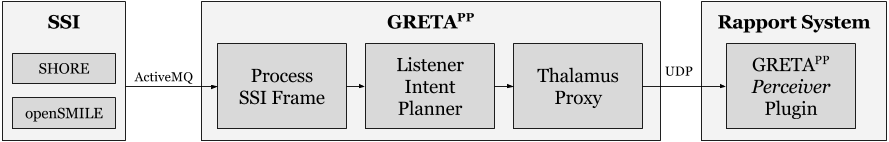
\includegraphics[width=0.47\textwidth]{figures/SupportingTechnologiesOverview.png}
	\caption{Schematic representation of the components that supports the rapport model.}
	\label{fig:SupportingTechnologiesOverview}
\end{figure}

GRETA\textsuperscript{PP} is a variation of the GRETA system~\cite{Niewiadomski2009} that contains solely its \textit{Listener Intention Planner} rule-based component that behaves identically to the rapport model's \textit{Backchannel} \textit{Effector}. The perceptions and the generated behaviour are sent to the GRETA\textsuperscript{PP} \textit{Perceiver} Plugin using \ac{UDP} sockets so that it notifies the interested \textit{Effectors}. The system has a slight delay ($<$ 1 second), as the refresh rate had to be halved to 5Hz so that the system could handle the resource heavy \ac{SSI}.

The following \textit{Effectors}' parameters were parametrised empirically following several pilots on 3 different people. The generated action proposals have the priority of 1, with the exception of Backchannel \textit{Effector} that has priority of 2 as it is not considered an idle behaviour. Finally, the mimicry behaviour is only done once every 3500ms.

%%%%%%%%%%%%%%%%%%%%%%%%%%%%%%%%%%%%%%%%%%%%%%%%%%%%%%%%%%%%%%%%%%%%%%%%%%%%%%%%%%%%%%%%%%%%

\subsection{Facial Expression Mimicry}
\label{sub:sec:facialExpressionMimicryImplementation}

The Facial Expression Mimicry rapport \textit{Effector} mimics the user's emotion given SHORE's emotion with highest intensity. With the probability of 50\%, it proposes actions, as long as happiness, sadness, and anger intensities detected are 0.65, 0.65, and 0.5, respectively. Nonetheless, the implementation of this plugin is not without issues as SHORE was detecting happy emotions in absence of faces. We solved that issue by applying a smoothing signal at the cost of increasing the delay from less than 1 second, to at most 3 seconds. In the end, we opted to remove the smoothing filter and compensate with disabling it when the user was not present.

%TODO nao estou a falar das animacoes aleatorias

\subsection{Head Gestures Mimicry}

The Head Nod Mimicry \textit{Effector} proposes up-down nod gestures and left-right head shakes given Kinect's perceived head gesture. As the sensors seldom detected head gestures during the pilot tests, both gestures' probabilities are set to 1. In addition, it produces light head nods that are slightly randomised in each action proposal to avoid being repetitive.

\subsection{Mutual-Gaze}
The Mutual-Gaze \textit{Effector} swaps the gaze target depending on the current state of the interaction assuming that the user is extroverted (lowest standard deviation), as we are unable to know the personality beforehand. The gaze durations are the default values.

\subsection{Backchannel}
The Backchannel \textit{Effector} produces listener behaviour according to the GRETA system~\cite{Niewiadomski2009}, proposing up-down head nods actions.  However, we were unable to reduce the impact of noise (agent's robotic movement and voice) on the \ac{SSI} sensors, leading to excessive false positives. Despite the attempts of counteracting the issue through noise-suppressing directional microphones and adjusting the sensors' parameters, the issue persisted, therefore the Backchannel \textit{Effector} was not used during the studies.
\section{Studies}
\label{sec:studies}

The developed rapport system was tested using the Quick Numbers scenario (Figure~\ref{fig:quickNumbersScenario}) regarding likeability, intelligence and liveness using the Godspeed series~\cite{bartneck2009measurement, lehmann2015good}, and
	Proximity~\cite{aron1992inclusion}.

\begin{figure}[H]
	\centering
	\frame{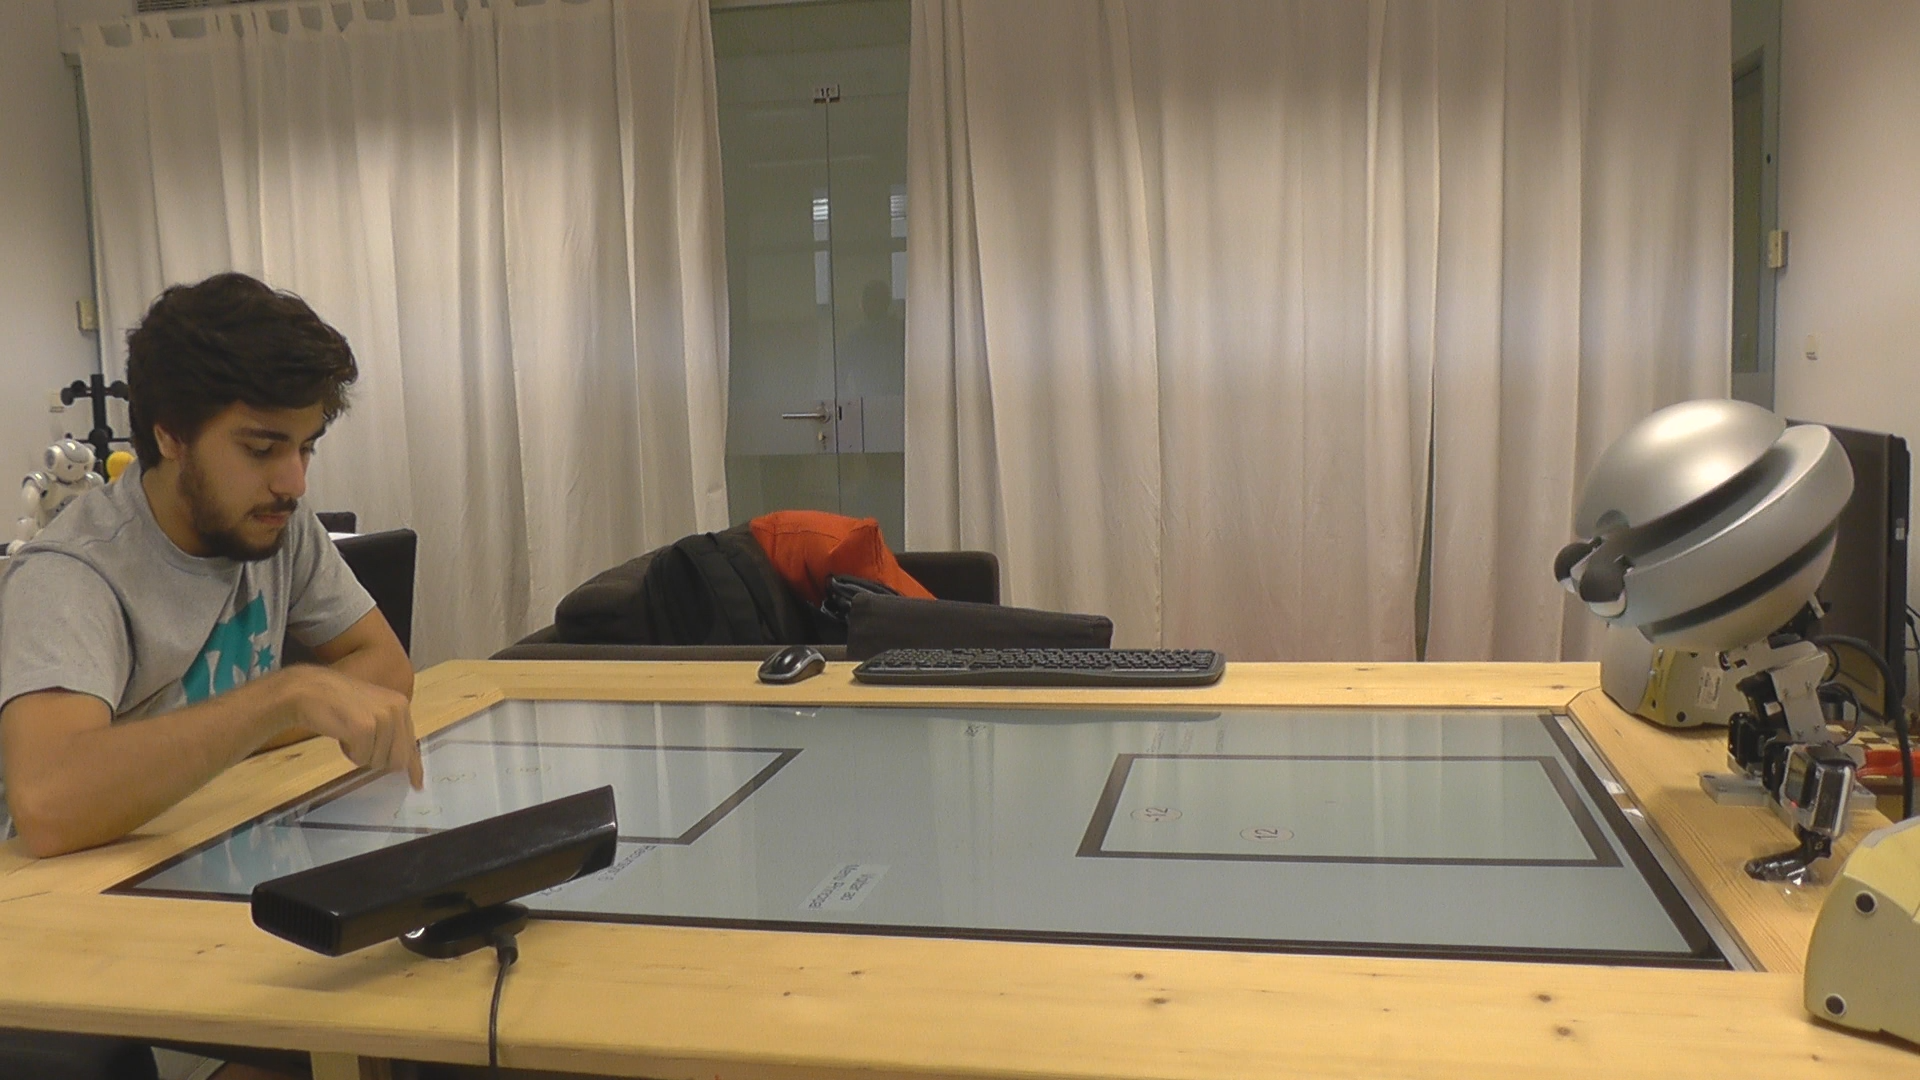
\includegraphics[width=0.35\textwidth]{ScenarioScreenShot.png}}
	\caption{An example of a participation in the Quick Numbers study (side view).}
	\label{fig:quickNumbersScenario}
\end{figure}

\subsection{Quick Numbers}

In the Quick Numbers scenario players are tasked with gaining as many resources as possible within the given time. At the beginning, each player starts with a fixed amount of resources that can be invested before each round. Depending on the amount invested and the player's performance, the returning investment will either be greater or lesser than the investment. The task is to tap the appearing numbers in sequential order starting with number one until the end of the round (Figure~\ref{fig:quickNumbers}). With each successful tap, the score increases, and with each incorrect number, the score decreases. In the end, the resources earned are the product between the amount invested and the round's score.

In this study, \ac{EMYS} accompanies the subject throughout the scenario, not as an opponent, but as another player that is also playing the game. The scenario stages go as follow:
\begin{itemize}
	\item \textbf{Introduction}: brief explanation of the rules, followed by the start the scenario;
	\item \textbf{Training Stage}: the participant plays an informal match alone to get accustomed to the game mechanics;
	\item \textbf{Gaming Session}: both players play a single round, at the same time;
	\item \textbf{Results Discussion}: the agent comments the each player scores;
	\item \textbf{Investment}: the participant is informed that he has to invest on the agent;
	\item \textbf{Ending}: \ac{EMYS} informs the value of the investment return and thanks to the subject for his participation.	
\end{itemize}

\begin{figure}[H]
	\centering
	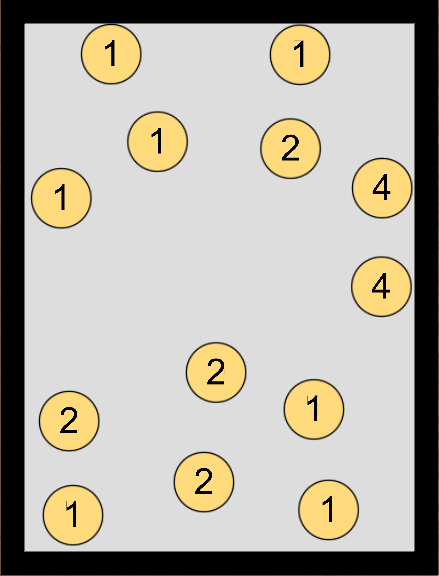
\includegraphics[width=0.2\textwidth]{FallingBoltsDiagram.png}
	\caption{Illustration of the Quick Numbers game developed in Unity.}
	\label{fig:quickNumbers}
\end{figure}

\subsection{Quick Numbers Plugins}

In addition to the plugins that implements the rapport model, we developed the following:
\begin{itemize}
	\item \textbf{Scenario \textit{Perceiver}}: monitors the scenario through \textit{Thalamus}, notifying the interested \textit{Effectors};
	\item \textbf{Utterances Manager}: proposes utterances according to the dyadic state of the interaction;
	\item \textbf{Rapport Strategies Manager}: enables/disables the rapport \textit{Effectors} throughout the scenario; 
\end{itemize}

The Utterances Manager \textit{Effector} implements the Positivity rapport \textit{Effector} and satisfies the ``Adhere to Social Norms'' goal of the rapport model by proposing utterances tailored to Quick Numbers (Table~\ref{fig:extended:utterances}). As the participant speaks Portuguese, different utterances are used depending on the subject's gender.

The Rapport Strategies Manager \textit{Effector} disables postural mimicry and mutual gaze rapport strategies during the Gaming Session and Investment stages, when \ac{EMYS} participates in Quick Numbers as a player and not as a spectator. In particular, it disables Facial Expression Mimicry \textit{Effector} in the investment phase because the participant's face is not visible on the video feed.

%This \textit{Effector} implements the positivity and the coordination component of the rapport model, proposing utterances according to the dyadic state of the interaction following the same structure as Table~\ref{fig:extended:utterances}. Given that \ac{EMYS} and the participant speak Portuguese, different utterances are used depending on the participant's gender. In addition to greeting and dismissing the participant, the rapport agent also: shares that it played sueca recently~\cite{correia2016trust}; motivates and praises the participant's performance; attempts to be humorous by saying ``I won't go anywhere... how could I? I am just a head...''.

\subsection{Results}
\label{sec:results}

A group of 40 participants from different universities campus participated in this study. The participants were equally selected and randomly distributed between the control condition (C) and the rapport condition (R), making two independent groups. Condition C has a mean age of 23.5±1, equal distribution of genders, and over 55\% of the participants already interacted with \ac{EMYS}. Condition R has a mean age of 25.65±3.945, 60\% male and only 25\% of the sample played with \ac{EMYS} in the past.

The study follows a between-subjects design, using significance level of 5\% for every statistical analysis.

\subsection*{\textbf{\textit{Are the rapport strategies effective in making agents more likeable?}}}

From the questionnaires, we compared the likability statistics between condition C (Figure~\ref{fig:likability_baseline}) and R (Figure~\ref{fig:likability_rapport}). As the distributions do not follow a normal distribution on both conditions ($sig_C=0.001$ and $sig_R=0$), we compare them with the \textit{Mann–Whitney U} statistical test. As the histogram's shapes are dissimilar ($sig=0.201$), we can only compare the mean scores: 5.0±0.649 and 5.3±0.865, on conditions C and R, respectively.

\begin{figure}[ht]
	\centering
	\begin{minipage}[b]{.2\textwidth}
		\centering
		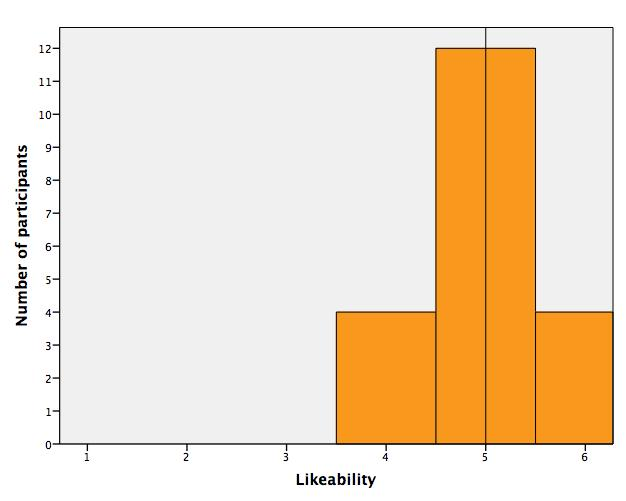
\includegraphics[width=\textwidth]{LikabilityBaseline.jpeg}
		\caption{Likeability histogram in the control condition.}
		\label{fig:likability_baseline}
	\end{minipage}
	\hspace{2mm}
	\begin{minipage}[b]{.2\textwidth}
		\centering
		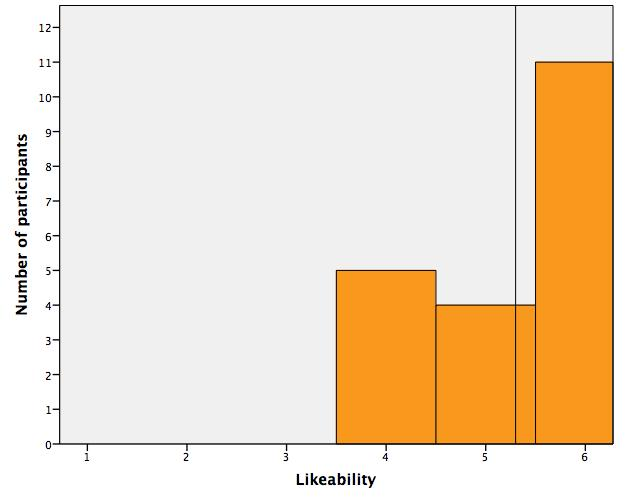
\includegraphics[width=\textwidth]{LikabilityRapport.jpeg}
		\caption{Likeability histogram in the rapport condition.}
		\label{fig:likability_rapport}
	\end{minipage}
\end{figure}



\textbf{Answer}: Despite the greater man average on the rapport condition, there is no statistical proof that rapport strategies are effective on increasing likeability. However, given that the mode (most frequent value) changed from 5 to 6, from condition C to condition R, we can postulate that, if we increase the sample size, we might obtain a clear confirmation that the rapport strategies affect the agent's likeability.


\subsection*{\textbf{\textit{Does the developed system improve agent's liveness?}}}

Similar to likeability, the animacy distribution on both conditions does not follow a normal distribution ($sig_C=0.002$ and $sig_R=0.003$), therefore we compare them using the \textit{Mann–Whitney U} statistical test. As the histograms' shapes (Figures~\ref{fig:animacy_baseline} and~\ref{fig:animacy_rapport}) are distinct ($sig=0.512$), we can only compare the mean scores: 4.25±0.716 and 4.3±1.031, on conditions C and R, respectively.

\begin{figure}[ht]
	\centering
	\begin{minipage}[b]{.2\textwidth}
		\centering
		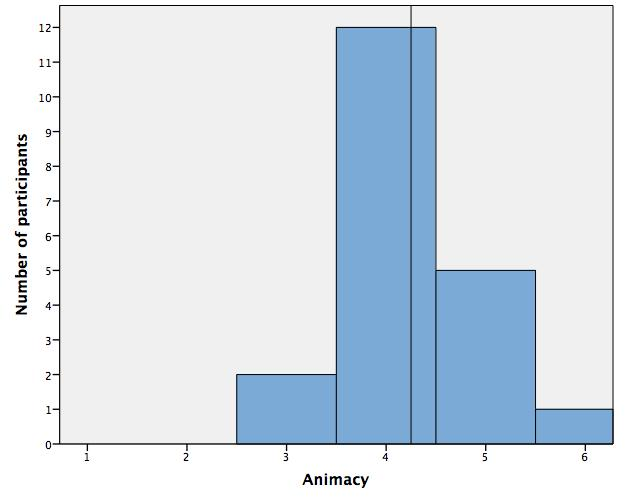
\includegraphics[width=\textwidth]{AnimacyBaseline.jpeg}
		\caption{Animacy histogram in the control condition.}
		\label{fig:animacy_baseline}
	\end{minipage}
	\hspace{2mm}
	\begin{minipage}[b]{.2\textwidth}
		\centering
		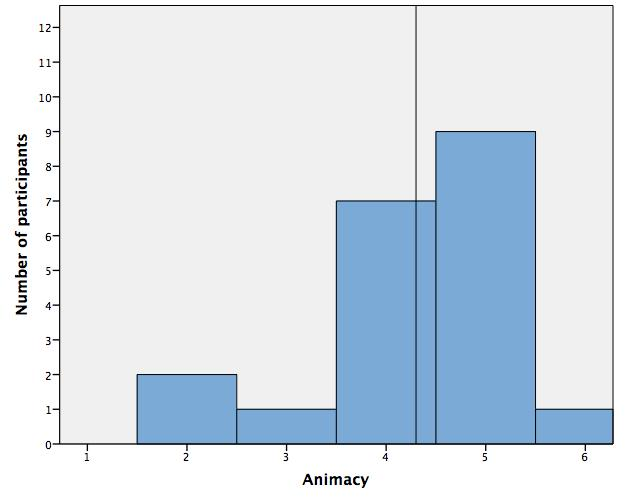
\includegraphics[width=\textwidth]{AnimacyRapport.jpeg}
		\caption{Animacy histogram in the rapport condition.}
		\label{fig:animacy_rapport}
	\end{minipage}
\end{figure}

\textbf{Answer}: There is no definite proof that the current system improves the agent's liveness.

\subsection*{\textbf{\textit{Do rapport strategies affect the perceived intelligence?}}}

Similar to likeability and animacy, the perceived intelligence distributions on  conditions C and R are not normal ($sig_C=0$ and $sig_R=0.002$), therefore we compare both conditions with the \textit{Mann–Whitney U} statistical test. The histogram's shapes (Figures~\ref{fig:intelligence_baseline} and~\ref{fig:intelligence_rapport}) are dissimilar ($sig=1.0$), therefore we only compare the mean scores: 5.1±0.553 and 5.0±0.918, on conditions C and R, respectively.

\begin{figure}[H]
	\centering
	\begin{minipage}[b]{.2\textwidth}
		\centering
		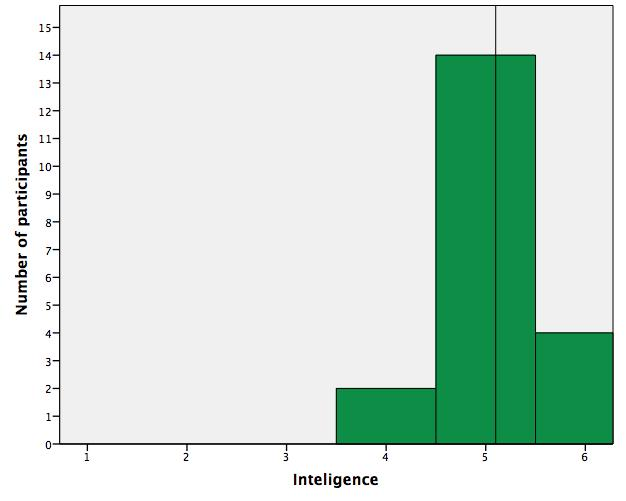
\includegraphics[width=\textwidth]{PerceivedIntelligenceBaseline.jpeg}
		\caption{Perceived intelligence histogram in the control condition.}
		\label{fig:intelligence_baseline}
	\end{minipage}
	\hspace{2mm}
	\begin{minipage}[b]{.2\textwidth}
		\centering
		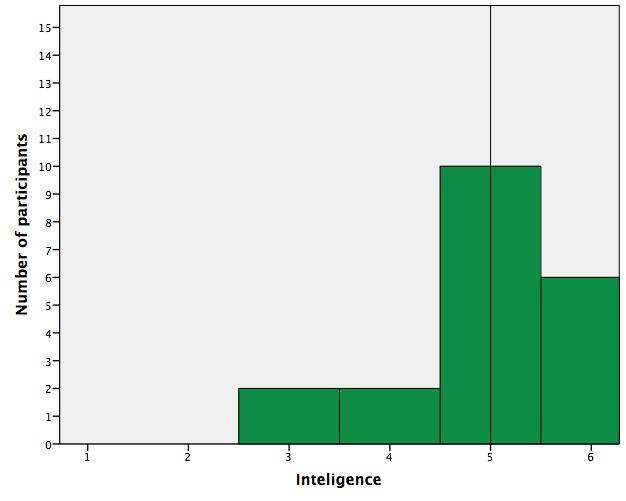
\includegraphics[width=\textwidth]{PerceivedIntelligenceRapport.jpeg}
		\caption{Perceived intelligence histogram in the rapport condition.}
		\label{fig:intelligence_rapport}
	\end{minipage}
\end{figure}


\textbf{Answer}: There is no statistical proof that the rapport strategies have an effect on the agent's perceived intelligence.
 
\subsection*{\textit{\textbf{Are the rapport strategies effective in establishing closer relationships between humans and agents?}}}

In order to answer the last hypothesis, we compare the proximities answers between conditions C (Figure~\ref{fig:proximity_baseline}) and R (Figure~\ref{fig:proximity_rapport}) using a 7-item scale question. In both conditions, proximity follows a normal distributions ($sig_C=0.203$ and $sig_R=0.304$), therefore we use the independent \textit{t-test} statistic test which yielded the statistical significance value of 0.694 ($>0.05$), consequently we reject the null hypothesis.

\begin{figure}[ht]
	\centering
	\hspace{5mm}
	\begin{minipage}[b]{.2\textwidth}
		\centering
		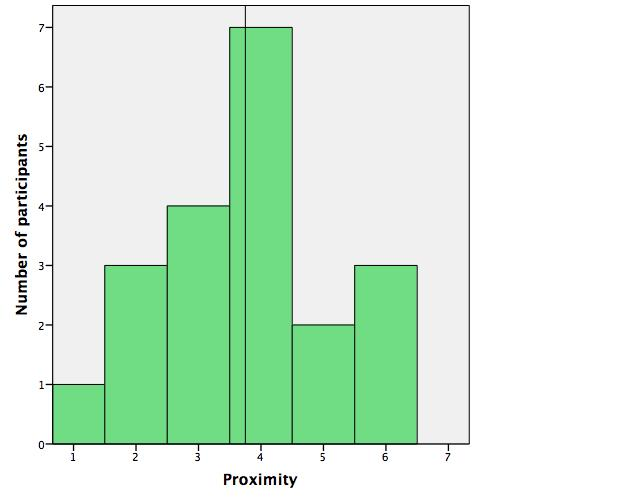
\includegraphics[width=\textwidth]{EmysBaseline.jpeg}
		\caption{Proximity histogram in the control condition.}
		\label{fig:proximity_baseline}
	\end{minipage}
	\hspace{2mm}
	\begin{minipage}[b]{.2\textwidth}
		\centering
		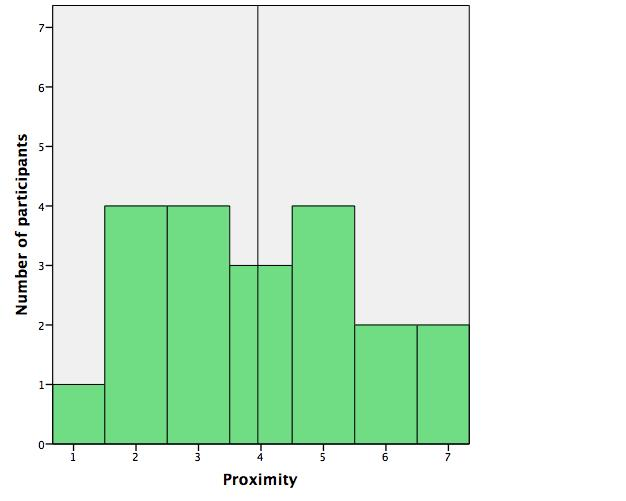
\includegraphics[width=\textwidth]{EmysRapport.jpeg}
		\caption{Proximity histogram in the rapport condition.}
		\label{fig:proximity_rapport}
	\end{minipage}
\end{figure}


\textbf{Answer}: Despite the small increase of 0.2 on the mean score from condition C to R, the impact of the rapport strategies on proximity are inconclusive.
\fancychapter{Conclusions}
\label{chap:conclusions}

This dissertation addresses the development of a rapport model that enables robotic and virtual agents to show natural signs of rapport according to the dyadic state of the interaction. This work was inspired by current literature on rapport~\cite{Buschmeier2011, Spencer-Oatey2005, Zhao2014, Papangelis2014} and social agents~\cite{Zwiers2011, Reidsma2011, Riek2009, Niewiadomski2009, Andrist2014, Andrist2015, Cassell2007, Wang2009, Schroder2010, Buschmeier2011, Tullio2015}.

The main difficulties during the development of this dissertation were:
\begin{itemize}
	\item Gathering and organising current research on rapport and social agents onto a consistent computational model;
	\item Developing the framework that implements rapport model while maintaining compatibility with current \ac{SERA} agents;
	\item Integration of \ac{SSI}, SHORE, and GRETA with the developed framework;
	\item Designing the tools to assure that current researchers may start using the developed system.
\end{itemize}

The model is based on the development of decoupled rapport strategies that can be refined and customised individually, to any agent and \ac{HRI} scenario. The model was integrated using the \ac{SERA} ecosystem and tested using robot \ac{EMYS}, however, we had to create a framework within \ac{SERA} to support interruption and replacement of the agent's ongoing actions as required in the rapport model. The goal of the framework is to provide technical and non-technical researchers, the tools to design agents capable of showing signs of rapport. Several efforts were made so that the system maintained compatibility with \ac{SERA}, be customisable, and work with external tools such as \ac{SSI}, SHORE and GRETA thanks to the collaboration of Fraunhofer Institute for Integrated Circuits (IIS) and TELECOM ParisTech university. In fact, current \ac{SERA} agents can use the developed rapport model with low effort.

To conclude, there were no relevant conclusions from the Quick Numbers user studies regarding likeability, perceived intelligence, liveness and proximity. However, from the video footage, it was clear that participants had more positive reactions on the rapport condition than on the control condition. For this purpose, it is possible to retrieve additional behavioural metrics from the recorded video (total 1235 minutes) to analyse, for example, smile frequency and length of eye contact. In addition, from the histograms, despite the lack of statistically significant results on the obtained results, there is a clear pattern that rapport strategies can make the agents more likeable as intended, which may be confirmed by repeating the studies with a sample greater than 20.




%TODO escarrapachar as dificuldades?

\section{Contributions}
\label{sec:contributions}

This dissertation contributed to:
\begin{itemize}
    \item Design of a rapport model that enables robotic and virtual agents to show natural signs of rapport according to the dyadic state of the interaction;
    \item Construction of a framework that implements the rapport model and eases the development of rapport agents by technical and non-technical researchers;
    \item Integration of \ac{SSI}, SHORE and SEMAINE with the \ac{SERA} ecosystem using the developed framework as intermediary;
    \item Development of a novel scenario called Quick Numbers, to evaluate rapport and trust;
    \item User studies that evaluate a rapport agent using robot \ac{EMYS} regarding participant perception of likeability, animacy, intelligence and felt proximity.
\end{itemize}

\section{Future Work}

This section presents several ideas that can be implemented in the future, to improve the work developed so far.

First of all, we need to evaluate the system on a different scenario focused on rapport, not on trust with a greater sample. This would aim to shift the participant's focus from the game to the agents, which has impacted the reported results in this document. In addition, we should look into behavioural metrics such as eye contact and smile frequency.

Secondly, future versions of the rapport model should consider mechanisms to assess rapport success so that the agent might adapt his behaviours to the user and even recover from mistakes~\cite{Kahn2008}. For example, use SHORE to monitor the emotional state of the user and attempt use humour to cheer him as soon as sadness becomes the most average emotion. In addition, we should continue collaboration with Fraunhofer Institute for Integrated Circuits (IIS) so that we can continuously improve the rapport model and the system using the SHORE's perceptual capabilities. For example, estimate the user gender to automatically select the most appropriate set of utterances.

Thirdly, we should explore resumable actions, that is, explore agents capable of resuming their course of action after being interrupted by external stimuli.

Finally, the backchannel \textit{Effector} should be revisited as it is only lacking an improved noise suppressing mechanism. This plugin has the potential to greatly enhance mutual attention and coordination that are two of the three components of rapport. Looking ahead, this \textit{Effector} should explore current \ac{ML} models to generate listener behaviour, as the current literature suggests that data models are the key to generating more humanly social behaviours.

%\end{document}  % This is where a 'short' article might terminate

First of all, I would like to thank my family for their love and invaluable support, always making sure that my brain had the right amount of nutrients to work.

I would like to thank my advisors, Professor Ana Paiva and Professor Rui Prada, for their invaluable experience, expertise and guidance throughout the last year.

I'd also like to thank Tiago Ribeiro, Brian Ravenet, Sofia Petisca, Angelo Cafaro and Tobias Baur for their valuable support and prompt guidance during the development of this project. In addition, I would like to show my appreciation to Fraunhofer Institute for Integrated Circuits (IIS) and TELECOM ParisTech university for their collaboration on SHORE and GRETA, respectively.

A special thank you to my amazing friends, both inside and outside Instituto Superior Técnico, who provided the timely distractions and motivations. Special thanks to Nuno Xu for his invaluable collaboration during the development of the user studies, but, not the least, for being my friend. Another special thanks to Tiago Santos whose unique humour never fails to perplex me, always providing the right laugh at the right time. Special thanks to my closest friend Emanuel Lopes, who is currently doing his PhD and yet, took the time to review this document. In addition, in no particular order, I would like to thank Ana Apura, Frederico Sabino, Miguel Faria, Pedro Garcia, Joana Teixeira, Nuno Sousa, André Pires, and Rita Santos for being there for me.

Lastly, and not the least, this thesis would not be possible without my caring and loving girlfriend, Joana Pinto, who was always there for me and whose idiosyncratic stubbornness proved invaluable when reviewing the dissertation. 

Thank you.
%
% The following two commands are all you need in the
% initial runs of your .tex file to
% produce the bibliography for the citations in your paper.
\bibliographystyle{abbrv}
\bibliography{bib/sigproc, bib/questionnaires, bib/library}

% This is "Appendices.tex"
%\balancecolumns
\appendix

\section{Framework Screenshots}

\begin{figure}[H]
	\centering
	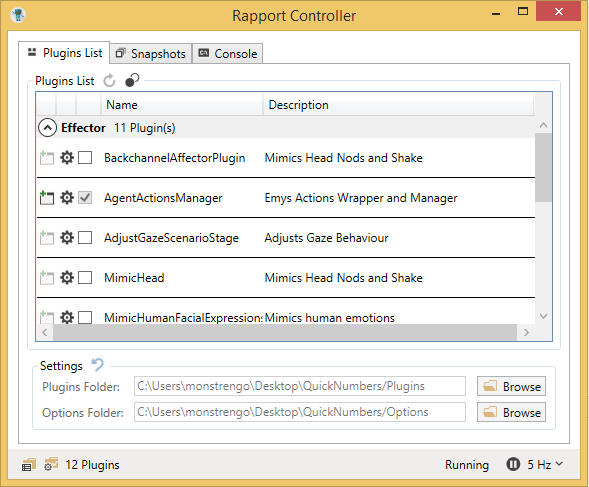
\includegraphics[width=0.47\textwidth]{PluginsList.png}
	\caption{\ac{GUI} representation of the system.}
	\label{fig:pluginList}
\end{figure}

\begin{figure}[H]
	\centering
	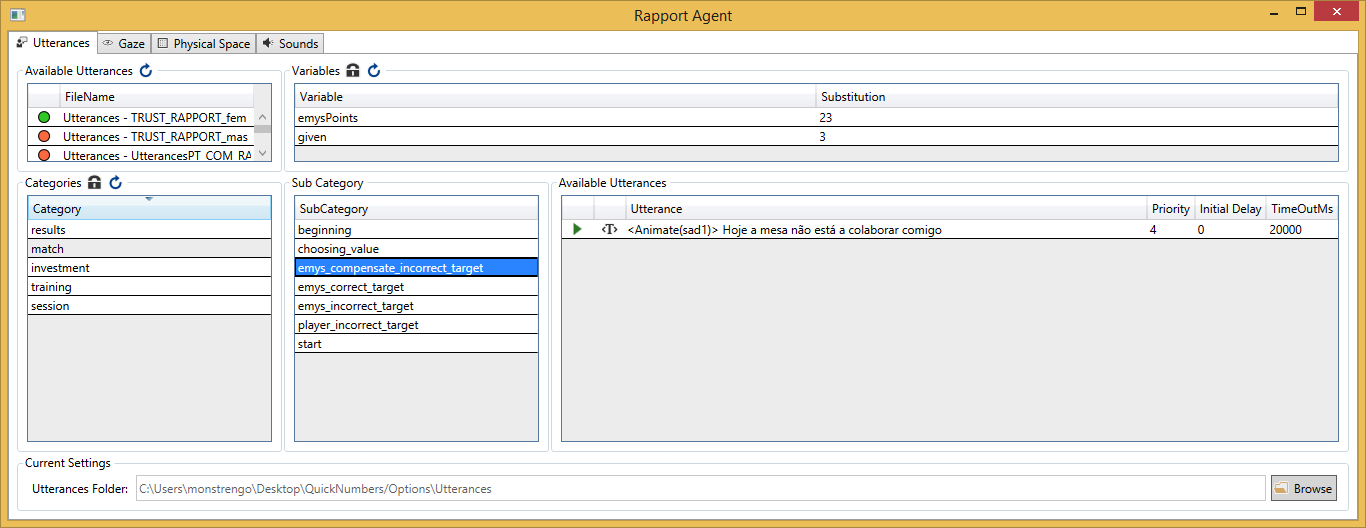
\includegraphics[width=0.47\textwidth]{ScreenshotAgentsManager.png}
	\caption{\ac{GUI} representation of the Agent Action Manager \textit{Utility} plugin.}
	\label{fig:agentActionsManagerScreenshot}
\end{figure}

%TODO verificar onde é que s\ao mencionadas as figuras

%\balancecolumns % GM June 2007
\end{document}
